\documentclass[12pt]{article}
\newcommand{\mybibstyle}{plain}

% dummy commands to make the whole thing sorta work
\newcommand{\email}[1]{}
\newcommand{\homepage}[1]{}
\newcommand{\affiliation}[1]{}
\newcommand{\pacs}[1]{}
\newenvironment{acknowledgments}{\paragraph*{Acknowledgements}}{}

\usepackage{amsmath}
\usepackage{amssymb}
\usepackage{bm}
\usepackage{booktabs}
\usepackage{color}
\usepackage{graphicx}
\usepackage{hyperref}
\usepackage{natbib}
\usepackage{siunitx}
\usepackage{subfigure}

\newcommand{\D}{\operatorname{d\!}}
\newcommand{\E}{\operatorname{e}}
\newcommand{\bra}[1]{\langle #1 |}
\newcommand{\braket}[2]{\langle #1 | #2\rangle}
\newcommand{\ket}[1]{| #1 \rangle}
\newcommand{\normord}[1]{\mathopen: #1 \mathclose:}

\begin{document}
\title{Studies of quantum dots}

\author{Fei Yuan}
\email{yuan@nscl.msu.edu}
\homepage{https://people.nscl.msu.edu/~yuan}
\affiliation{National Superconducting Cyclotron Laboratory and Department of Physics and Astronomy, Michigan State University, East Lansing, MI 48824, USA}
\author{J\o rgen H\o gberget}
\affiliation{Department of Physics, University of Oslo, N-0316 Oslo, Norway}
\author{Sam Novario}
\affiliation{National Superconducting Cyclotron Laboratory and Department of Physics and Astronomy, Michigan State University, East Lansing, MI 48824, USA}
\author{Nathan Parzuchowski}
\affiliation{National Superconducting Cyclotron Laboratory and Department of Physics and Astronomy, Michigan State University, East Lansing, MI 48824, USA}
\author{Sarah Reimann}
\affiliation{Department of Chemistry and Center for Theoretical and Computational Chemistry, University of Oslo, N-0316 Oslo, Norway}
\author{Scott Bogner}
\affiliation{National Superconducting Cyclotron Laboratory and Department of Physics and Astronomy, Michigan State University, East Lansing, MI 48824, USA}
\author{Morten Hjorth-Jensen}
\affiliation{National Superconducting Cyclotron Laboratory and Department of Physics and Astronomy, Michigan State University, East Lansing, MI 48824, USA}
\affiliation{Department of Physics, University of Oslo, N-0316 Oslo, Norway}

\begin{abstract}
  We present and compare several many-body methods used to study a quantum dot system.  We calculate the approximate ground state energy of electrons in a circularly symmetric potential well using a harmonic oscillator basis optimized via Hartree-Fock (HF).  We further improve the ground state energy using in-medium similarity renormalization group (IM-SRG).  Additionally, we calculate the addition and removal energies using quasidegenerate perturbation theory (QDPT).  Our results are benchmarked against quasi-exact diffusion Monte Carlo (DMC) and coupled cluster (CC) calculations.
\end{abstract}

\pacs{02.70.Ss, 31.15.A-, 31.15.bw, 71.15.-m, 73.21.La}
\maketitle

\section{Introduction}

Understanding the behavior of strongly confined electrons is of fundamental
interest for solving many-body problems.  Quantum dots, e.g. electrons
confined in semiconducting heterostructures, are of particular interest since
they exhibit, due to their small size, discrete quantum levels.  Under these
conditions, typical quantum phenomena like tunneling, entanglement and
magnetization can all be observed \cite{reimann2002,engel1993}.  Since quantum
dots are manufactured and designed artificially at the laboratory, their
quantum levels can be arbitrarily tuned by changing the external field or the
size and shape of the system.  As a consequence, quantum dots provide a high
level of control for the dynamics and correlation of the electrons, which
makes them perfectly suited to study quantum effects in practice.  Since their
ground state shows similar shell structures and magic numbers as seen for
atoms and nuclei \cite{tarucha1996}, these systems give the opportunity to
study electronic systems without the presence of a nucleus affecting the
electrons.  Apart from their relevance for theoretical research in quantum
physics, quantum dots offer a wide variety of applications: In particular,
their electrical and optical properties make them attractive for the use in
laser technology \cite{strauf2010,5075760} and solar cells
\cite{jenks:013111,doi:10.1021/cr900289f}, but they are also used in quantum
computers\cite{PhysRevA.57.120} and medical imaging \cite{Ben-Ari02042003}.

In order to properly understand the properties of quantum dots and make
theoretical predictions of their behavior in various applications, it is
necessary to study features like ground state energy and correlation
effects. Since there generally does not exist an analytical solution for
quantum dots except for ones containing only two electrons or with specific
values of the external field \cite{PhysRevA.48.3561}, the development of
appropriate numerical few- and many-body methods is required to solve the
problem.

Several \textit{ab initio} methods have been applied to these systems, in
particular variational and diffusion Monte Carlo (VMC and DMC)
\cite{PhysRevB.68.035304,%
  PhysRevB.62.8120,PhysRevB.84.115302,PhysRevB.54.4780}, large-scale
diagonalization/full configuration interaction (FCI)
\cite{JJAP.36.3924,PhysRevB.56.6428,2008arXiv0810.2644K,rontani:124102} and coupled
cluster (CC) theory \cite{PhysRevB.67.045320,heidari:114708,%
  PhysRevB.84.115302}.

Additionally to those approaches, another very promising first-principles
method has recently been developed.  The similarity renormalization group
(SRG) is a family of methods that drives the Hamiltonian toward a band- or
block-diagonal form through a continuous sequence of unitary transformations,
reducing the coupling between a subspace of interest -- such as the ground
state -- and the remaining Hilbert space.  It has successfully been applied to
study systems with different underlying potentials and to analyse their
binding energy and other observables, especially in nuclear theory
\cite{ScottSRG,PhysRevC.75.061001,SRGThreeDim}.  Aside from usual
\emph{free-space} SRG, where the Hamiltonian is constructed with respect to
the vacuum state with no physical particles, it is possible to evolve a
Hamiltonian via SRG \emph{in medium} through the normal-ordering technique,
which enables the Hamiltonian to be constructed with respect to some reference
state containing a finite number of particles.  In-medium SRG (IM-SRG) can
further take advantage of the normal-ordering process to account for 3-body
forces in an approximate manner without resorting to the full, computationally
intensive 3-body machinery.  The method allows considerable simplifications to
the problem and makes numerical calculations much more efficient \cite{IMSRG}.

This article is organized as follows: Section \ref{sec:formalism} introduces
first (\ref{subsec:modelHamiltonian}) the Hamiltonian we use to model circular
quantum dots, and gives afterwards an overview of the IM-SRG
(\ref{subsec:imsrgmethod}) and DMC (\ref{subsec:DMC}) formalisms.  Our results are
presented in Section \ref{sec:results}.  We point out the differences arising
from the use of two different generators (Wegner and White generator), and
give an overview of the ground state energies up to 42 particles. In
particular, we compare the results obtained with five different \textit{ab
  initio} methods: IM-SRG(2), DMC, Hartree-Fock, FCI and CC. Section
\ref{sec:conclusions} concludes our work and gives perspectives for future
work.

The harmonic oscillator (HO) is a ubiquitous system in quantum physics. It is the basis for an extremely diverse set of many-body calculations -- in nuclear physics \cite{HJORTHJENSEN1995125}, quantum chemistry \cite{helgaker2000molecular}, and quantum dot calculations of solid state physics \cite{reimann2002}. In these calculations, one typically seeks a few of the lowest eigenvalues $E_k$ and eigenvectors of a many-body Hamiltonian $\hat{H}$ that describes the full system by solving the Schr\"odinger equation,
\begin{equation*}
\hat{H} \ket{\psi_k} = E_k \ket{\psi_k}, \quad k \in \{1, 2, \ldots, k_{\text{max}}\}.
\end{equation*}
In all cases, the many-body wave function is expanded in a basis of
eigenstates of the one-body HO system.  Necessarily, in order to perform
numerical calculations the basis must be truncated to give an approximation.
In particular, the so-called ``curse of dimensionality'' implies that for a
system with many particles the number of available degrees of freedom per
particle is severely limited by the finiteness of a computer.

[[This paragraph seems to be talking about a different paper]]
It is clear, that an understanding of the properties of such expansions,
giving \emph{a priori} error estimates on many-body calculations, is very
important. Unfortunately, this is a neglected topic in the physics
literature. In this article, we give a thorough mathematical and numerical
analysis and give practical convergence estimates of HO basis expansions. It
generalizes and refines the findings of a recent study of one-dimensional
systems.\cite{Kvaal2007}

The HO eigenfunctions are popular for several reasons. Many quantum systems, such as the quantum dot model considered here, can be considered perturbed harmonic oscillators \textit{per se}, thus the true eigenstates should be perturbations of the HO eigenstates.  Moreover, the HO has many beautiful properties, such as separability, invariance under orthogonal coordinate changes, and easily computable eigenfunctions, so that computing matrix elements of relevant operators becomes relatively simple.  Since HO eigenfunctions are defined on the \emph{entire} space in which particles live, a truncation of the spatial domain is unnecessary.  This avoids one of the main problems with approaches such as finite difference or finite element methods.\cite{ram2002finite} [[Unknown citation]]

\section{Formalism}
\label{sec:formalism}

\subsection{The model Hamiltonian}
\label{subsec:modelHamiltonian}

We shall model the circular quantum dot system as a collection of $N$ nonrelativistic electrons of mass $m$ in 2-dimensional space, trapped by an external harmonic-oscillator potential of the form $m \omega^2 r^2 / 2$, where $\omega$ is the angular frequency of the oscillator trap and $r$ is the distance from the center of the trap.  The electrons interact with each other through the standard Coulomb interaction $e^2 / (4 \pi \epsilon R)$, where $e$ is the charge of each electron, $\epsilon$ is the permittivity of the medium, and $R$ is the distance between the two interacting electrons.

Even though the model system contains 5 parameters $(N, m, \omega, e, \epsilon)$, many of them are redundant.  With an appropriate choice of units, the number of parameters in the system can be reduced to just two.  For rest of this paper, we shall use atomic units\footnote{Here, ``atomic unit'' is used in an \emph{abstract} sense: we do not assume (nor care) whether $m$, $e$, $\epsilon$ correspond to true values in vacuum, or some effective value in medium.} where $\hbar$, $m$, $e$ and $4 \pi \epsilon$ all have a value of one.  Hartree $E_{\mathrm{h}}$ becomes the unit of energy and the Bohr radius $a$ becomes the unit of length:
\begin{align*}
  E_{\mathrm{h}} &\equiv m \left(\frac{e^2}{4 \pi \epsilon \hbar}\right)^2 &
  a &\equiv \frac{4 \pi \epsilon \hbar^2}{m e^2}
\end{align*}
This leaves us with $(N, \omega)$ as the only parameters necessary to specify the quantum dot system, with $\omega$ in units of $E_{\mathrm{h}} / \hbar$.

The behavior of each electron in isolation is described by the kinetic energy $t(\bm{r})$ and the potential energy due to the trap $u(\bm{r})$, which combine to form the standard harmonic oscillator Hamiltonian $h(\bm{p}, \bm{r})$:
\begin{align*}
  t(\bm{p}) &\equiv \frac{1}{2} \bm{p}^2 &
  u(\bm{r}) &\equiv \frac{1}{2} \omega^2 \bm{r}^2 &
  h(\bm{p}, \bm{r}) &\equiv t(\bm{p}) + t(\bm{r})
\end{align*}
Here, $\bm{p}$ is the linear momentum of the electron and $\bm{r}$ is its position relative to the center of the trap.  The pairwise interaction between two electrons at positions $\bm{r}$ and $\bm{r}'$ is simply the Coulomb interaction:
\begin{align*}
  v(\bm{r}, \bm{r}') \equiv \frac{1}{|\bm{r} - \bm{r}'|}
\end{align*}
Then, the full many-body problem is described by the Hamiltonian
\begin{align*}
  \hat H \equiv \hat H^{[1]} + \hat H^{[2]}
\end{align*}
where $\hat{H}^{[1]}$ and $\hat{H}^{[2]}$ are the one- and two-body parts of the Hamiltonian,
\begin{align} \label{eq:onetwobodyhamiltonian}
\hat{H}^{[1]} &\equiv \sum_{j = 1}^N h(\hat{\bm p}_j, \hat{\bm r}_j) &
\hat{H}^{[2]} &\equiv \sum_{j_1 = 1}^N \sum_{j_2 = 1}^{j_1 - 1} v(\hat{\bm r}_{j_1}, \hat{\bm r}_{j_2})
\end{align}
The operator $\hat{\bm r}_j$ is the position operator of the $j$-th particle,\footnote{The ordering of the particle labels $j$ is unimportant as they exist only for the purpose of bookkeeping.} and $\hat{\bm p}_j \equiv -\mathrm{i} \hat{\bm{\nabla}}_{\bm{r}_j}$ is its momentum operator.

\begin{figure}
  % [width=.48\textwidth]
  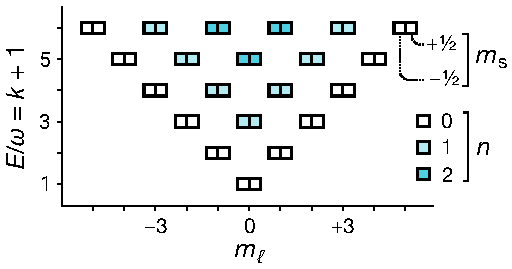
\includegraphics[width=\textwidth]{figures/fig-shell-structure-v2}
  \caption{Visualization of the 20 lowest single-particle states in the 2D harmonic oscillator basis.  Each box represents a single-particle state arranged by $m_\ell$, $m_{\mathrm{s}}$, and energy, and the up/down arrows indicate the spin of the states.  The $n$ quantum number increases upward vertically, starting at zero for the lowest state within a each column.}
  \label{fig:shell-structure}
\end{figure}

The noninteracting part of the many-body Hamiltonian $\hat{H}^{[1]}$ can be reduced to $N$ independent single-particle Hamiltonians each of the form:
\begin{align*}
  \hat{h} = \frac{1}{2} \hat{\bm{\nabla}}^2 + \frac{1}{2} \omega^2 \hat{\bm{r}}^2
\end{align*}
Therefore, solving the noninteracting many-body problem amounts to solving the single-particle Schr\"odinger equation
\begin{align*}
  \hat{h} |p\rangle = \varepsilon_p |p\rangle
\end{align*}
where $p$ is an unknown tuple of quantum numbers.  The two-dimensional harmonic oscillator Hamiltonian $\hat{h}$ has well known analytic solutions in Cartesian coordinates, but for our purposes, we prefer to use the Fock-Darwin states, which favor a representation in polar coordinates $\bm{r} = (\rho, \varphi)$ and have the useful property of conserving the orbital angular momentum $\hat{L}_{\mathrm{z}} \equiv -\mathrm{i} \partial / (\partial \varphi)$.

The Fock-Darwin wave functions can be decomposed into radial and angular components,\cite[Appx.\ A]{lohne2010coupled}
\begin{align}
  F_{n, m_\ell}(\rho, \varphi) &\equiv \sqrt\omega R_{n, |m_\ell|}(\sqrt \omega \rho) A_{m_\ell}(\varphi) \label{eq:fockdarwin} \\
  R_{n, m}(\varrho) &\equiv \sqrt{\frac{2 \cdot n!}{(n + m)!}} \mathrm{e}^{-\varrho^2 / 2} \varrho^m L_n^{(m)}(\varrho^2) \notag \\
  A_{m_\ell}(\varphi) &\equiv \frac{1}{\sqrt{2 \pi}} \mathrm{e}^{\mathrm{i} m_\ell \varphi} \notag
\end{align}
where $L_n^{(m)}$ denotes the generalized Laguerre polynomial of degree $n$ and parameter $m$,
\begin{align*}
  L_n^{(m)}(u) = \frac{1}{n!} u^{-m} \mathrm{e}^u \frac{\mathrm{d}^n}{\mathrm{d} u^n} (\mathrm{e}^{-u} u^{m + n})
\end{align*}
The states are labeled by two quantum numbers: the principal quantum number $n \in \{0, 1, \ldots\}$ and the orbital angular momentum projection $m_\ell \in \mathbb Z$, which is the eigenvalue of $\hat{L}_{\mathrm{z}}$.

Since electrons are spin-$1/2$ fermions, they can occupy either of the two possible spin states $\chi_{-1/2}$ or $\chi_{+1/2}$.  The complete single-particle basis state $| (n, m_\ell, m_{\mathrm{s}}) \rangle$ contains both a spatial component \eqref{eq:fockdarwin} and a spin component,
\begin{align} \label{eq:singleparticlestate}
  \langle (\rho, \varphi) | (n, m_\ell, m_{\mathrm{s}}) \rangle \equiv F_{n, m_\ell}(\rho, \varphi) \chi_{m_{\mathrm{s}}}
\end{align}
where we have introduced the the spin projection $m_{\mathrm{s}} \in \bigl\{-1/2, +1/2\bigr\}$ as the third quantum number.

The energy of the single-particle state $\phi_{n, m_\ell, m_{\mathrm{s}}}$ is given by
\begin{align*}
  \varepsilon_{n, m_\ell, m_{\mathrm{s}}} \equiv (2 n + |m_\ell| + 1) \omega
\end{align*}
The energies are degenerate with respect to the spin projection $m_{\mathrm{s}}$ as our Hamiltonian $\hat{h}$ does not distinguish between them.  Additionally, they are degenerate with respect to the nonnegative integer
\begin{align} \label{eq:shell_index}
  k \equiv 2 n + |m_\ell|
\end{align}
which we conveniently call the \textit{shell index} as it labels each shell starting from zero.  The shells are equidistant with an energy spacing equal to the frequency $\omega$.

Going back to the many-body Hamiltonian $\hat{H}^{[1]}$, we can use the Slater determinant construction to build an $N$-particle eigenstate $|p_1, \ldots, p_N\rangle$ of the many-body Hamiltonian $\hat{H}^{[1]}$ from an arbitrary choice of $N$ single-particle eigenstates $|p_1\rangle, \ldots, |p_N\rangle$ from \eqref{eq:singleparticlestate}, where $p$ is an abbreviation of the triplet $(n, m_\ell, m_{\mathrm{s}})$.  It is important to emphasize that a Slater determinant $|p_1, \ldots, p_N\rangle$ is not merely a product of the single-particle states, but an antisymmetrized sum over all possible products,
\begin{align*}
  \langle \bm{r}_1, \ldots, \bm{r}_N | p_1, \ldots, p_N \rangle \equiv
  \frac{1}{\sqrt{N}} \left|
  \begin{matrix}
    \langle \bm{r}_1 | p_1 \rangle & \cdots & \langle \bm{r}_1 | p_N \rangle \\
    \vdots & \ddots & \vdots \\
    \langle \bm{r}_N | p_1 \rangle & \cdots & \langle \bm{r}_N | p_N \rangle \\
  \end{matrix}
  \right|
\end{align*}
The Slater determinant $|p_1, \ldots, p_N\rangle$ is said to \textit{occupy} the states $|p_1\rangle, \ldots, |p_N\rangle$.  By construction, Slater determinants satisfy the Pauli exclusion principle, ensuring that the exchange of any two particles is equivalent to a reversal in the sign of the many-body wave function.

The energy of a Slater determinant is given by a sum over the occupied single-particle energies,
\begin{align*}
  \hat{H}^{[1]} | p_1, \ldots, p_N \rangle = (\varepsilon_{p_1} + \cdots + \varepsilon_{p_N}) | p_1, \ldots, p_N \rangle
\end{align*}
It is possible for Slater determinants occupying different sets of single-particle states to be degenerate in energy.  This is possible even for ground states of $\hat{H}^{[1]}$.  However, if the number of particles $N$ satisfies $N = K_{\mathrm{F}} (K_{\mathrm{F}} + 1)$ for some nonnegative integer $K_{\mathrm{F}}$, there would be just enough particles to form a closed-shell Slater determinant, leading to a unique, well-isolated ground state.  The values of $N$ at which this occurs are said to be \textit{magic numbers}.  We call $K_{\mathrm{F}}$ the \textit{number of filled shells} (or ``Fermi level'').  In particular, a single-particle state is occupied in the ground state Slater determinant if and only $k < K_{\mathrm{F}}$, where $k$ is the shell index of the single-particle state as defined in \eqref{eq:shell_index}.

Currently, the Hamiltonian $\hat{H}$ is explicit in the number of particles $N$.  The many-body machinery can be made agnostic to number of particles through the formalism of second quantization, similar to quantum field theory.  The many-body Hilbert space is extended from states with only $N$ particles to states with every possible number of particles via the Fock space construction.  Slater determinants can then rewritten as,
\begin{align*}
  |p_1, \ldots, p_N\rangle =
  \hat a_{p_1}^\dagger \cdots \hat a_{p_N}^\dagger |\rangle
\end{align*}
whre $|\rangle$ is the \textit{vacuum state} -- the unique state that is devoid of particles -- and $\hat{a_p}^\dagger$ denotes a \textit{creation operator} for the single-particle state $p$.  If the single-particle state $p$ is not yet occupied by a particle, $\hat a_p^\dagger$ adds such a particle to the state.  Otherwise, it collapses the entire many-body state to the number $0$ (not to be confused with the vacuum state $|\rangle$).  The Hermitian conjugate of $\hat a_p^\dagger$ is \textit{annihilation operator} $\hat a_p$, which has the opposite effect of removing the particle if it exists, collapsing to zero otherwise.  For fermions, the field operators $\hat a_p$ and $\hat a_p^\dagger$ satisfy the essential anticommutation relations,
\begin{align*}
  &\{\hat a_p, \hat a_q\} = \{\hat a_p^\dagger, \hat a_q^\dagger\} = 0 &
  &\{\hat a_p, \hat a_q^\dagger\} = \delta_{p, q}
\end{align*}
where $\delta_{p, q}$ denotes the Kronecker delta.

In second quantization, the one- and two-body Hamiltonian operators $H^{[1]}$ and $\hat{H}^{[2]}$ from \eqref{eq:onetwobodyhamiltonian} can be rewritten as\footnote{The reversed ordering of $\hat a_s \hat a_r$ here is completely intentional.}
\begin{align} \label{eq:second_quantized_hamiltonian}
  \hat H^{[1]} &= \sum_{p, q} \langle p | \hat{H}^{[1]} | q \rangle \hat a_p^\dagger \hat a_q^{} &
  \hat{H}^{[2]} &= \frac{1}{4} \sum_{p, q, r, s} \langle p, q | \hat{H}^{[2]} | r, s \rangle \hat a_p^\dagger \hat a_q^\dagger \hat a_s^{} \hat a_r^{}
\end{align}
where the numbers $\langle p | \hat{H}^{[1]} | q \rangle$ and $\langle p, q | \hat{H}^{[2]} | r, s \rangle$ are known as \textit{matrix elements}, whose values fully characterize the operators.  In this paper, we use the letters $p, q, r, s, t, \ldots$ as labels for arbitrary single-particle basis states.  In the harmonic oscillator basis, the letters can be considered abbreviations for triplets of the form $(n, m_\ell, m_{\mathrm{s}})$.  A summation such as $\sum_p$ is to be understood as a summation over every single-particle basis state $p$.  This is very different from \eqref{eq:onetwobodyhamiltonian}, where summations such as $\sum_j$ are performed over arbitrary particle \emph{labels}.  We thus see another benefit with second quantization: the Hamiltonian representation does not distinguish particles at all, as it should be for quantum particles.

The complete Hamiltonian is given by the sum
\begin{align}
  \hat{H} = \sum_{p, q} \langle p | \hat{H}^{[1]} | q \rangle \hat{a}_p^\dagger \hat{a}_q + \frac{1}{4} \sum_{p, q, r, s} \langle p, q | \hat{H}^{[2]} | r, s \rangle \hat{a}_p^\dagger \hat{a}_q^\dagger \hat{a}_r \hat{a}_s  \label{eq:vacuumhamiltonian}
\end{align}
Due to the antisymmetry of Slater determinants, we have the property that exchanging either $p$ with $q$ or $r$ with $s$ causes $\langle p, q | \hat{H}^{[2]} | r, s \rangle$ to reverse in sign, leading to a 4-fold symmetry that is canceled out by the factor of $1/4$.  For this reason, the two-body matrix element $\langle p, q | \hat{H}^{[2]} | r, s \rangle$ is commonly referred to as the \emph{antisymmetrized} matrix element.  This is not to be confused with the non-antisymmetric interaction integral,
\begin{align*}
  v_{p_1, p_2, p_3, p_4} \equiv \int \langle \bm{r} | p_1 \rangle \langle \bm{r}' | p_2 \rangle v(\bm r, \bm r') \langle \bm{r} | p_3 \rangle \langle \bm{r}' | p_4 \rangle \D \bm{r} \D \bm{r}'
\end{align*}
This object only has a 2-fold symmetry: $v_{p_1, p_2, p_3, p_4} = v_{p_2, p_1, p_4, p_3}$.  The antisymmetrized matrix element can be computed from the interaction integral via
\begin{align*}
  \langle p, q | \hat{H}^{[2]} | r, s \rangle = v_{p, q, r, s} - v_{p, q, s, r}
\end{align*}

In our work, the interaction integrals $v_{p, q, r, s}$ were computed numerically using the algorithm presented in \cite{2008arXiv0810.2644K}, included as part of the OpenFCI program.  The algorithm uses numerical quadrature to calculate the integrals exactly in the center-of-mass frame and then performs a transformation to obtain matrix elements in the laboratory frame.  The numerical quadrature technique is much more numerically robust and efficient than using analytical formulas such as the one in \cite{0953-8984-10-3-013}.

The use of second quantization allows the application of a powerful combinatoric theorem known as Wick's theorem \cite{shavitt2009many}, which provides systematic way to expand complicated expressions involving creation and annihilation operators.  Ultimately, computations \textit{in silico} do not involve algebraic manipulation of abstract operators at all -- rather, they involve numerical calculations of \emph{matrix elements} via equations derived using Wick's theorem.

With the basic formalism and notation established, we begin discussion of techniques to solve the full many-body Hamiltonian $\hat H$.  The difficulty stems from the fact that the exact solution cannot be expressed in terms of a single Slater determinant due to the presence of interactions.  Hence, it is not possible to trivially reduce the problem to that of a single particle as we had done previously.

However, if we assume the interaction alters the behavior of the system to only a mild extent, we can use Slater determinants of the noninteracting system as starting points for the full solution, and then apply various many-body methods to improve the accuracy of the solution.

\subsection{Hartree-Fock method}
\label{subsec:HartreeFockmethod}

One relatively simple correction that we can apply to our solution is that of the Hartree-Fock (HF) method.  Using the variational principle, we compute an approximate ground state $\Phi$ by minimizing the energy expectation value
\begin{align*}
  E_{\Phi} \equiv \langle \Phi | \hat H | \Phi \rangle
\end{align*}
with respect to $\Phi$, subject to the restriction that $\Phi$ is a single Slater determinant constructed from an unknown set of $N$ orthonormal single-particle states.  We denote each unknown single-particle state $|q'\rangle$ by a primed label $q'$.

To make this computationally feasible, we further assume that each unknown state $|q'\rangle$ can be built from a linear combination of known states, $|p\rangle$ for all $p$.  This reduces the problem from an abstract mathematical one to a numerical linear algebra problem, with the caveat that this set of known functions be large enough to ensure convergence.

Assuming the interaction is not too strong, we can use the single-particle states of our noninteracting Hamiltonian as a basis for the unknown states.  The two sets of states are then related by a linear transformation matrix $\bm C$:
\begin{align*}
  |q'\rangle = \sum_p |p\rangle C_{p, q'}
\end{align*}
To ensure the orthonormality of the states, we assume the set of unknown states $|q'\rangle$ has as many elements as the set of known states $|p\rangle$ and we require the coefficient matrix $\bm C$ to be unitary.  While these conditions are more strict than necessary, they greatly simplify the calculations and allow the states $|q'\rangle$ to act as inputs for methods beyond HF.  The set of states $|q'\rangle$ now consists of $N$ \textit{occupied} states that participate in the Slater determinant $\Phi$ and the remaining \textit{unoccupied} states that do not.

Since the coefficient matrix uniquely determines the unknown states, the variational problem has been reduced to that of solving of the coefficients $\bm C$ that minimize the energy $E_{\Phi}$, which is given by
\begin{align}
  E_{\Phi} &= \sum_{j} n_j H^{[1] \prime}_{j, j} + \sum_{j, k} n_j n_k H^{[2] \prime}_{j, k, j, k} \label{eq:hfenergy}
\end{align}
where the transformed operators are defined as
\begin{align}
  H^{[1] \prime}_{p, q} &\equiv \sum_{r, s} C_{r, p}^* \langle r | H^{[1]} | s \rangle C_{s, q}^{} \label{eq:hftransform1} \\
  H^{[2] \prime}_{p, q, r, s} &\equiv \sum_{t, u, v, w} C_{t, p}^* C_{u, q}^* \langle t, u | H^{[2]} | v, w \rangle C_{v, r}^{} C_{w, s}^{} \label{eq:hftransform2}
\end{align}
and the occupancy number $n_p$ is defined as
\begin{align}
  n_p \equiv \begin{cases}
    1 & \text{if $p$ is an occupied state in $\Phi$} \\
    0 & \text{if $p$ is an unoccupied state in $\Phi$}
  \end{cases}
\end{align}
and further define $\bar n_p \equiv 1 - n_p$ as the complement.

With the method of Lagrange multipliers, the minimization problem can be reduced to the solving of a nonlinear equation -- the \textit{Hartree-Fock equation}:
\begin{align} \label{eq:hartreefock}
  \bm F \bm C = \bm C \bm \epsilon
\end{align}
where the \textit{Fock matrix} $\bm F$ is defined as
\begin{align} \label{eq:fock}
  F_{p, q} \equiv H_{p, q}^{[1]} + \sum_{r, s, j} n_j C_{r, j}^* V_{p, r, q, s}^{} C_{s, j}^{}
\end{align}
and $\bm \epsilon$ is a vector of Lagrange multipliers with each element $\epsilon_q$ associated with a particular state $|q'\rangle$.

The HF equation can be solved by an iterative technique: a solution $\bm C$ can be fed into \eqref{eq:fock} and new solution can then obtained by solving the eigenvalue problem in \eqref{eq:hartreefock} using the Fock matrix obtained.  For the initial guess, we use the ground state of our noninteracting Hamiltonian, thus $\bm C$ is initially the identity matrix.  After dozens of iterations, perhaps with the aid of a convergence acceleration technique (such as DIIS [[cite??] or Broyden's method [[cite?]]), one would usually reach a state of self-consistency where the solution converges to a fixed value.  This is the Hartree-Fock solution.

Since HF restricts the ground state to a Slater determinant of single-particle
states, it cannot provide an exact solution to a problem where correlations
are present even if the single-particle basis is not truncated (infinite in size).  The
energy difference between the best Hartree-Fock energy and the exact ground
state energy is thus by definition known as the \textit{correlation energy}.
The focus of post-HF methods such as IM-SRG is to improve on the HF results,
thus recovering parts of this missing energy.

To make use of the HF solution as the reference state for future calculations, we transform the operators via \eqref{eq:hftransform1} and \eqref{eq:hftransform2}.  Therefore, the post-HF methods described in the next few sections generally use the transformed operators $\hat{H}^{[1] \prime}$ and $\hat{H}^{[2] \prime}$ as inputs.  However, for generality, we omit the prime symbols as the methods do not necessitate a state optimized by HF.

\subsection{The IM-SRG method}
\label{subsec:imsrgmethod}

\subsubsection{Similarity renormalization group methods}
\label{subsubsec:srgmethods}

In similarity renormalization group (SRG) methods, one performs a continuous
sequence of unitary transformations on a Hamiltonian operator $\hat H$ to
evolve it into a band- or block-diagonal form, reducing the coupling between a
small model space of interest from its complementary space.  This allows the
Hilbert space to be truncated to the small model space without losing
significant accuracy.

The sequence of transformations is parameterized by a continuous variable $s$
known as the \textit{flow parameter}.  By convention we define to be $0$ at
the beginning of the sequence, and thus the evolving Hamiltonian $\hat H(s)$
at $s = 0$ is set to the original Hamiltonian.  Upon reaching $s$, the
transformed Hamiltonian is given by
\begin{align*}
  \hat H(s) \equiv \hat U(s) \hat H(0) \hat U^\dagger(s)
\end{align*}
where $U(s)$ is a unitary operator that describes the product of all such
transformations since $s = 0$.  Taking the derivative with respect to $s$, we obtain:
\begin{align*}
  \frac{\D}{\D s} H(s) =
  \left(\frac{\D}{\D s} \hat{U}(s)\right) \hat{H}(0) \hat{U}^\dagger(s) +
  \hat{U}(s) \hat{H}(0) \frac{\D}{\D s} \hat{U}^\dagger(s)
\end{align*}
If we define an operator $\eta(s)$ as
\begin{align*}
  \eta(s) \equiv \left(\frac{\D}{\D s} \hat{U}(s)\right) \hat{U}^\dagger(s)
\end{align*}
we find that it is antihermitian as a result of the unitarity of $\hat{U}(s)$:
\begin{align*}
  \eta(s) + \eta^\dagger(s)
  = \frac{\D}{\D s} \left(\hat{U}(s) \hat{U}^\dagger(s)\right)
  = 0
\end{align*}
From this property we can derive a differential equation known as the
\textit{SRG flow equation}:
\begin{align} \label{eq:imsrgode}
  \frac{\D}{\D s} H(s) = [\eta(s), \hat{H}(s)]
\end{align}
The equation allows $\hat{H}(s)$ to be evaluated without explicitly
constructing the full transformation $\hat U(s)$.  The operator $\hat \eta(s)$
is known as the \textit{generator} of the transformation.  When ``integrated''
as a product, the full transformation $\hat U(s)$ is recovered:
\begin{align*}
  \hat U(s')
  = \mathcal T_s \left\{ \mathrm{e}^{\int_0^{s'} \hat{\eta}(s) \D s} \right\}
  \equiv \lim_{\Delta s \to 0} \prod_{s = 0, \Delta s, \ldots}^{s = s'}
  \mathrm{e}^{\hat \eta(s) \Delta s}
\end{align*}
Here $\mathcal T_s$ is a notational device that denotes $s$-ordering: a reordering of the $\hat{\eta}(s)$ operator products expanded from the exponential with respect to $s$ in ascending order \cite[\S 6.1]{reimann2013quantum}.  This is analogous to the usual time-ordering from quantum field theory.

The operator $\hat{\eta}$ can be chosen to suppress certain undesirable parts of the Hamiltonian matrix, which can be considered the ``off-diagonal'' parts in a loose sense.  The ``off-diagonal'' parts could be elements far away from the matrix diagonal, in which case the evolution drives the matrix towards a band-diagonal form.  Or, the ``off-diagonal'' parts could be elements that couple the ground state from the excited state, in which case the evolution drives the matrix towards a block-diagonal form that isolates the ground state.  Or, the ``off-diagonal'' could be literally the elements that do not lie on the diagonal, in which case the evolution would simply diagonalize the Hamiltonian.  Through different choices of $\hat{\eta}$, the SRG evolution can be controlled and adapted to the features of a particular problem.

\subsubsection{Evolving the flow equation in medium}

The SRG flow equation \eqref{eq:imsrgode} can be solved in the second quantization formalism described in Section \ref{subsec:modelHamiltonian}, where field operators are defined with respect to the physical vacuum state.  However, since the size of the problem grows enormously with the number of particles and the size of the model space, the applicability of this free-space SRG method is restricted to comparatively small systems.  Alternatively, the evolution can be done at finite density, i.e.\ directly in an $N$-particle system defined by a reference state \cite{kehrein2006flow}.  This gives rise to the IM-SRG method.

The second-quantized operators in \eqref{eq:second_quantized_hamiltonian} are constructed with respect to the vacuum state.  That is, the operator strings $\hat{a}_p^\dagger \hat{a}_q$ and $\hat{a}_p^\dagger \hat{a}_q^\dagger \hat{a}_s \hat{a}_r$ both have a vacuum expectation value of zero:
\begin{align*}
&\bra{\varnothing} \hat{a}_p^\dagger \hat{a}_q \ket{\varnothing} = 0 &
&\bra{\varnothing} \hat{a}_p^\dagger \hat{a}_q^\dagger \hat{a}_s \hat{a}_r \ket{\varnothing} = 0
\end{align*}
They are said to be \emph{normal-ordered} with respect to the vacuum state $\varnothing$.  It is possible to be normal-ordered with respect to a non-vacuum state, however.  Consider a Slater determinant $\Phi$ with $N_{\mathrm{F}}$ occupied states:
\begin{align*}
  \ket{\Phi} \equiv \ket{\varnothing_{i_1, i_2, \ldots, i_{N_{\mathrm{F}}}}}
\end{align*}
where $\{i_1, i_2, \ldots, i_{N_{\mathrm{F}}}\}$ is a set of $N_{\mathrm{F}}$ indices that label the occupied states.  One can define a set of \textit{quasiparticle field operators} $\hat b$ and $\hat b^\dagger$ that obey the same anticommutation relations as the $\hat a$ operators:
\begin{align*}
  \hat b_p \equiv \bar n_p \hat a_{p} + n_p \hat a_{p}^\dagger
\end{align*}
The quasiparticle field operators treat $\ket{\Phi}$ as their ``vacuum state'' (sometimes called ``Fermi vaccuum'' in an abstract sense), despite not being the physical vacuum state.  As before, it is possible to construct arbitrary Slater determinants by applying quasiparticle operators to the reference state:
\begin{align}
  \ket{\Phi_{p_1, \ldots, p_k}} \equiv \hat{b}^\dagger_{p_1} \cdots \hat{b}^\dagger_{p_k} \ket{\Phi}
  \label{eq:quasisd}
\end{align}
If $p$ is an unoccupied state, then applying $\hat{b}_p^\dagger$ creates a particle exactly like $\hat{a}_p^\dagger$.  However, if $p$ is an occupied state, then applying $\hat{b}_p^\dagger$ destroys an existing particle in $\Phi$ or, equivalently, creates a \textit{hole} state.  The set of labels $\{p_1, \ldots, p_k\}$ may contain up to $N$ hole states and a potentially infinite number of particle states.  It is typical to classify the state $\Phi_{p_1, \ldots, p_k}$ as an $N_{\text{p}}$-particle-$N_{\text{h}}$-hole state, meaning that it contains $N_{\text{p}}$ labels that denote unoccupied states and $N_{\text{h}}$ labels that denote occupied states.  If $N_{\text{p}} = N_{\text{h}}$, the Slater determinant represents a system containing the same number of physical particles.

We may then define \emph{normal ordering with respect to the reference state} $\Phi$, a notational device that rearranges a string of operators such that every quasiparticle creation operator appears before a quasiparticle annihilation operator by repeatedly exchanging neighboring operators, with each exchange incurring a change in sign.  A simple example would be the normal ordering of a pair of field operators such as:
\begin{align*}
  \normord{\hat{b}_p \hat{b}_q^\dagger} =
  -\hat{b}_q^\dagger \hat{b}_p
\end{align*}
Here, we denote normal ordering of an operator string with respect to $\Phi$ by a pair of colons.  The expectation value of a normal ordered string of operators with respect to $\Phi$ is guaranteed to vanish:
\begin{align*}
&\bra{\Phi} \hat{b}_p^\dagger \hat{b}_q \ket{\Phi} = 0 &
&\bra{\Phi} \hat{b}_p^\dagger \hat{b}_q^\dagger \hat{b}_s \hat{b}_r \ket{\Phi} = 0
\end{align*}
The normal ordering of the quasiparticle field operators are straightforward to compute, but what is more interesting is the normal ordering of the physical field operators $\hat a$ and $\hat a^\dagger$ with respect to $\Phi$:
\begin{align*}
  \normord{\hat{a}_p^\dagger \hat{a}_q} &=
  \hat{a}_p^\dagger \hat{a}_q - n_p \delta_{p, q}
\end{align*}
The normal ordering notation thus provides a concise way of expressing the right-hand side.  In this new notation, we can rewrite the Hamiltonian $\hat H = \hat{H}^{[1]} + \hat{H}^{[2]}$ in its \emph{normal-ordered representation}:
\begin{align}
  \hat{H} = H^{[0]} + \sum_{p, q} H^{[1]}_{p, q} \normord{\hat{a}_p^\dagger \hat{a}_q} + \frac{1}{4} \sum_{p, q, r, s} H^{[2]}_{p, q, r, s} \normord{\hat{a}_p^\dagger \hat{a}_q^\dagger \hat{a}_r \hat{a}_s}
  \label{eq:normordhamiltonian}
\end{align}
where
\begin{align*}
  H^{[0]} &\equiv \sum_{i} n_i H^{[1]}_{i, i} + \frac{1}{2} \sum_{i, j} n_i n_j V_{i, j, i, j} \\
  H^{[1]}_{p, q} &\equiv H^{[1]}_{p, q} + \sum_{i} n_i V_{p, i, q, i} \\
  H^{[2]}_{p, q, r, s} &\equiv V_{p, q, r, s} \\
\end{align*}
If $\Phi$ is a state optimized by the HF method, then $H^{[0]}$ is simply the HF energy $E_\Phi$ and $H^{[1]}_{p, q}$ is the Fock matrix $F_{p, q}$.  The normal-ordered representation of $\hat H$ in \eqref{eq:normordhamiltonian} is completely equivalent to that of $\hat H$ in \eqref{eq:vacuumhamiltonian}.  The only difference is that it rearranges the matrix elements so as to emphasize the reference state $\Phi$ rather than vacuum state $\ket{\varnothing}$.  This makes a critical difference when the expressions containing 3-body or higher terms are \emph{truncated} to only 2-body.  If the reference state $\Phi$ is good approximation of the true solution $\Psi$, then the importance of the higher-body parts of the Hamiltonian are greatly reduced.

Higher-body operators arise from integrating the flow equations (\ref{eq:imsrgode}), which is one of the major challenges of the SRG method.  With each evaluation of the commutator, the Hamiltonian gains terms of higher order, and these induced contributions will in subsequent integration steps feed back into terms of lower order.  Thus, the higher-body contributions are not irrelevant to the final solution even if only the ground state energy is of interest.

Computationally, higher-body terms are difficult to handle: the amount of memory required to store an $r$-body operator is grows exponentially with $r$.  Moreover, the flow equations are capable of generating an infinite number of higher-body terms as the Hamiltonian evolves.  Thus, to make the method tractable, we must close the IM-SRG flow equations, truncating the equations to a finite order.

In this paper, we truncate both $\hat{H}$ and $\hat{\eta}$ at the two-body level, an approach known as IM-SRG(2).  This normal-ordered two-body approximation appears to be sufficient in many cases and has yielded excellent results for several nuclei \cite{PhysRevLett.106.222502,PhysRevLett.109.052501,IMSRG}.

Note that the loss of three-body and higher-body terms (\textit{operator truncation}) is only one out of the two sources of error in this method.  The other source of error is due to the \textit{basis truncation}, as with any method that relies on a finite single-particle basis.  The latter can be reduced by increasing the size of the basis at the expense of greater computational effort.

With the operator truncation, the generator $\hat{\eta}$ can be written as a generic antihermitian 2-body operator:
\begin{align*}
\hat{\eta} = \sum_{p, q} \eta_{p, q}^{[1]} \normord{\hat a_p^\dagger \hat a_q} +
\frac{1}{4} \sum_{p, q, r, s}\eta_{p, q, r, s}^{[2]} \normord{\hat a_p^\dagger \hat a_q^\dagger \hat a_s \hat a_r}
\end{align*}
where $\eta_{p, q}^{[1]}$ and $ \eta_{p, q, r, s}^{[2]}$ respectively are its one- and two-body matrix elements normal ordered with respect to $\Phi$.

By expanding the commutator in \eqref{eq:imsrgode} without consideration of the three-body term, we obtain the matrix-element form of the IM-SRG(2) flow equation:
\begin{align}
    \frac{\D H^{[r]}}{\D s} = C^{[r]}(\eta, H) \label{eq:flowmxe}
\end{align}
where
\begin{align}
  C^{[r]}(A, B) &\equiv 2 \mathcal{A}_{A, B} D^{[r]}(A, B) \text{ for any $r$, $A$, $B$} \label{eq:commutmxe} \\
  \mathcal{A}_{x, y} f(x, y) &\equiv \frac{1}{2} \bigl(f(x, y) - f(y, x)\bigr) \text{ for any $x$, $y$, $f$}
\end{align}
and finally
\begin{align}
  D^{[0]}(A, B)
  &\equiv
    \sum_{i, a} n_i \bar{n}_a A^{[1]}_{i, a} B^{[1]}_{a, i}
    + \frac{1}{4} \sum_{i, j, a, b} n_i n_j \bar{n}_a \bar{n}_b A^{[2]}_{i, j, a, b} B^{[2]}_{a, b, i, j}
    \label{eq:flow0} \\
  D^{[1]}_{p, q}(A, B)
  &\equiv
    \sum_{r} A^{[1]}_{p, r} B^{[1]}_{r, q}
    - \frac{1}{2} \sum_{i, j, a} n_i n_j \bar{n}_a A^{[2]}_{i, j, a, q} B^{[2]}_{a, p, i, j}
    + \frac{1}{2} \sum_{i, a, b} n_i \bar{n}_a \bar{n}_b A^{[2]}_{i, p, a, b} B^{[2]}_{a, b, i, q}
    \notag \\
  &\hphantom{=}
    + \sum_{i, a} n_i \bar{n}_a \left(
    A^{[1]}_{i, a} B^{[2]}_{a, p, i, q}
    + A^{[2]}_{i, p, a, q} B^{[1]}_{a, i}
    \right)
    \label{eq:flow1} \\
  D^{[2]}_{p, q, r, s}(A, B)
  &\equiv
    \tilde{\mathcal{A}}_{p, q} \tilde{\mathcal{A}}_{r, s}
    \sum_{i, a} n_i \bar{n}_a A^{[2]}_{i, p, a, r} B^{[2]}_{a, q, i, s}
    + \frac{1}{2} \sum_{i, j} n_i n_j A^{[2]}_{i, j, r, s} B^{[2]}_{p, q, i, j}
    + \frac{1}{2} \sum_{a, b} \bar{n}_a \bar{n}_b A^{[2]}_{p, q, a, b} B^{[2]}_{a, b, r, s}
    \notag \\
  &\hphantom{=}
    + \sum_{t} \left(
    \tilde{\mathcal{A}}_{p, q} A^{[1]}_{q, t} B^{[2]}_{p, t, r, s}
    + \tilde{\mathcal{A}}_{r, s} A^{[2]}_{p, q, r, t} B^{[1]}_{t, s}
    \right)
    \label{eq:flow2}
\end{align}
\begin{figure}
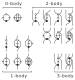
\includegraphics[width=.48\textwidth]{fig-diagrams-imsrg}
\caption{Diagrammatic representation of $C^{[r]}(\circ, \bullet)$ in \eqref{eq:commutmxe} that forms part of the IM-SRG flow equation \eqref{eq:flowmxe}.  The diagrams are implicitly antisymmetrized (Hugenholtz diagrams \cite{HUGENHOLTZ1957481} as described in \cite{shavitt2009many} \S 4.4.3).}
\label{fig:diagrams-imsrg}
\end{figure}
The equations can be derived directly from the anticommutation relations of the field operators, but it is more convenient to use Wick's theorem [[ref]] or, even more efficiently, diagrammatic techniques [[ref]] to arrive at the results.  In particular, the diagrammatic representation of antisymmetrized matrix elements are shown in Figure \ref{fig:diagrams-imsrg}.

An accurate and robust ODE solver is required to solve \eqref{eq:imsrgode}.  In particular, the solver must be able to handle the stiffness that can often arise (even in the case of White generator, which is designed to avoid some of the stiffness).  For our numerical experiments, we used a high-order ODE solver algorithm by L.\ F.\ Shampine and M.\ K.\ Gordon \cite{shampine1975computer}, which is a multistep method based on the implicit Adams predictor-corrector formulas.  Its source code is freely available \cite{odesolver}.

Through the flow equation and with an appropriate choice of the generator $\hat{\eta}$, the evolved state $\hat U(s) \ket{\Phi}$ will gradually approach a more ``diagonal'' form.  If the ``diagonal'' form decouples the ground state from the excited states, then $\hat U(\infty) \ket{\Phi}$ would yield the exact ground state solution of the problem if no operator or basis truncations are made.  In particular, $H^{[0]}$ would approach the true ground state energy.

The commutator in the flow equations \eqref{eq:imsrgode} indicates that the evolved state $\hat U(s) \ket{\Phi}$ can be expanded in terms of \emph{linked diagrams} only \cite{shavitt2009many,ISI:A1981MN73700014}, which ensures the size-extensive property of IM-SRG by construction.  This holds even if the commutator is truncated.  Regarding the quality of the SRG results, this indicates that the error introduced by truncating the many-body expansions scales linearly with the number of particles $N$.

\subsubsection{Wegner's canonical generator}
\label{subsec:Wegner}

To determine the specific unitary transformation, one needs to specify the generator $\hat{\eta}$.  Through different choices, the SRG flow can be adapted to the features of a particular problem.

The original choice suggested by Wegner \cite{Wegner200177} reads
\begin{equation}
  \hat{\eta}^{\text{Wg}}
  = [\hat{H}^{\text{d}}, \hat{H} - \hat{H}^{\text{d}}]
  = [\hat{H}^{\text{d}}, \hat{H}]
  \label{eq:etaWegner}
\end{equation}
where $\hat{H}^{\text{d}}$ denotes the ``diagonal'' part of the Hamiltonian (and $\hat{H} - \hat{H}^{\text{d}}$ denotes the ``off-diagonal'' part) in the abstract sense described at the end of section \ref{subsubsec:srgmethods}.

Since $\hat{\eta}^{\text{Wg}}$ is the commutator between two Hermitian operators, it is antihermitian as required for a generator.  Additionally, it can be shown that the commutator has the property of suppressing off-diagonal matrix elements as the state evolves via the flow equation \cite{kehrein2006flow}, as we would like.  In particular, matrix elements far off the diagonal, where the Hamiltonian couples states with large energy differences, are suppressed much faster than elements closer to the diagonal.

The matrix elements of the generator can be evaluated using \eqref{eq:commutmxe} to \eqref{eq:flow2}.  If define $\hat{H}^{\text{d}}$ via
\begin{align*}
  H^{\text{d}, [1]}_{p, q} &\equiv \delta_{p, q} H^{[1]}_{p, p} \\
  H^{\text{d}, [2]}_{p, q, r, s} &\equiv (\delta_{p, r} \delta_{q, s} - \delta_{p, s} \delta_{q, r}) H^{[2]}_{p, q, p, q}
\end{align*}
then the expressions for $\hat{\eta}^{\text{Wg}}$ can be simplified considerably:
\begin{align*}
  \eta^{\text{Wg},[0]} &= 0 \\
  \eta^{\text{Wg},[1]}_{p, q} &= 2 H^{[1]}_{p, q} \mathcal{A}_{p, q} \bigl( H^{[1]}_{p, p} + n_p H^{[2]}_{p, q, p, q} \bigr) \\
  \eta^{\text{Wg},[2]}_{p, q, r, s} &= 2 \mathcal{A}_{p, q} \mathcal{A}_{r, s} \Big( \\
  &\qquad H^{[2]}_{p, q, r, s} \mathcal{A}_{(p, q), (r, s)} \Bigl(\\
  &\qquad \qquad 2 H^{[1]}_{p, p} + 4 n_p H^{[2]}_{p, r, p, r} \\
  &\qquad \qquad + (1 - 2 n_p) H^{[2]}_{p, q, p, q} \Bigr) \\
  &\qquad + 4 \delta_{p, r} H^{[1]}_{q, s} \mathcal{A}_{(p, q), (r, s)} H^{[2]}_{p, q, p, q}
  \Bigr)
\end{align*}
where for any $x$, $y$, $z$, $w$, $f$ we define the antisymmetrizer
\begin{align*}
  \mathcal{A}_{(x, y), (z, w)} f(x, y, z, w) &\equiv \frac{1}{2} \bigl(f(x, y, z, w) - f(z, w, x, y)\bigr)
\end{align*}

\subsubsection{White generator}
\label{subsec:White}

Apart from Wegner's choice of the generator, there exist several other ones in literature. One choice, proposed by White \cite{White:cond-mat0201346}, makes numerical approaches much more efficient.  The problem with the Wegner generator is the widely varying decaying speeds of the Hamiltonian matrix elements.  Terms with large energy separations from the ground state are suppressed initially, followed by those with smaller energy separations.  This leads to stiffness in the flow equation, leading to numerical difficulties in solving the set of coupled differential equations.

White takes an alternative approach, which is especially suited for problems where one is interested in the ground state of a system.  Firstly, instead of driving all off-diagonal elements of the Hamiltonian to zero, he focuses solely on those ones that are connected to the reference state $\Phi$, aiming to decouple the reference state from the remaining Hamiltonian.  This reduces the amount of change performed on the Hamiltonian, which can reduce the accuracy loss resulting from the truncated higher-body terms.  Secondly, the rate of decay in Hamiltonian matrix elements are approximately normalized by dividing the generator matrix elements by an appropriate factor.  This reduces the stiffness of the flow equations.

The generator is explicitly constructed the following way \cite{PhysRevLett.106.222502,White:cond-mat0201346}
\begin{align*}
\hat{\eta}^{\text{Wh}} &\equiv \hat{\eta}' - \hat{\eta}'{}^\dagger
\end{align*}
where
\begin{align*}
\eta^{\prime [1]}_{a, i} &\equiv \frac{\bar{n}_a n_i H^{[1]}_{a, i}}{\Delta^{[1]}_{a, i}} &
\eta^{\prime [2]}_{a, b, i, j} &\equiv \frac{\bar{n}_a \bar{n}_b n_i n_j H^{[2]}_{a, b, i, j}}{\Delta^{[2]}_{a, b, i, j}}
\end{align*}
and the denominators $\Delta^{[1]}$ and $\Delta^{[2]}$ are
\begin{align*}
\Delta^{[1]}_{a, i} &\equiv H^{[1]}_{a, a} - H^{[1]}_{i, i} - H^{[2]}_{a, i, a, i} \\
\Delta^{[2]}_{a, b, i, j} &\equiv H^{[1]}_{a, a} + H^{[1]}_{b, b} - H^{[1]}_{i, i} - H^{[1]}_{j, j} + X_{a, b, i, j} \\
X_{a, b, i, j}
  &\equiv H^{[2]}_{a, b, a, b} - H^{[2]}_{a, i, a, i} - H^{[2]}_{b, i, b, i} \notag \\
  &\qquad + H^{[2]}_{i, j, i, j} - H^{[2]}_{a, j, a, j} - H^{[2]}_{b, j, b, j}
\end{align*}
These are the Epstein--Nesbet denominators.  Some literature use M\o eller--Plesset denominators, which omit the $X_{a, b, i, j}$ term, leading to a slightly different variant of the canonical White generator.

Compared to the Wegner generator, where the derivative of the final flow equations contain cubes of the Hamiltonian matrix elements (i.e.\ each term contains a product of 3 one-body and/or two-body matrix elements), the elements in White generators contribute only linearly.  This has reduces the stiffness in the differential equation, providing a net increase in computational efficiency since stiff ODE solvers tend to be slower and require more memory.

\subsection{Quasigenerate perturbation theory}
\label{subsec:selfenergy}

IM-SRG, in the approach described, provides a means to calculate the ground state energy of any system that is reasonably approximated by a single Slater determinant.  This works well for closed-shell systems, but it does not provide a direct means to obtain the ground state energy of open-shell systems.  While there exists more complicated multi-reference approaches to IM-SRG that can tackle the general problem \cite{Hergert2016165}, we opted to use the simpler quasidegenerate perturbation theory (QDPT), which provides us with a simple approach to extract ground state energies of open-shell systems that are only a few particles removed from a closed-shell system.  In particular, it allows us to calculate \textit{addition energies} $\epsilon_a$ and \textit{removal energies} $\epsilon_i$ of such systems, which we define as:
\begin{align}
  \epsilon_a &\equiv E_{\Phi_a} - E_{\Phi} \\
  \epsilon_i &\equiv E_{\Phi} - E_{\Phi_i}
\end{align}
where the meaning of $\Phi_p$ is defined in \eqref{eq:quasisd}, $i$ is restricted to labels of occupied states, and $a$ is restricted to labels of unoccupied states.

In QDPT, the solutions of the approximate Hamiltonian $\hat{H}^{[1]}$ are used as the basis of the model space.  One then assumes the existence of an operator $\hat \Omega$, known as the \textit{wave operator}, that maps some set of states $\tilde \Psi^{\mathrm{o}}_u$ within the model space to the exact ground state $\Psi_u$:
\begin{align} \label{eq:omega-condition1}
  \Psi_u = \hat \Omega \tilde \Psi^{\mathrm{o}}_u
\end{align}
The states $\tilde \Psi^{\mathrm{o}}_u$ consist of some mixture of the eigenstates
$\Psi^{\mathrm{o}}_{u'}$ of the approximate Hamiltonian $\hat{H}^{[1]}$.

There is some freedom in the choice of the wave operator $\hat \Omega$.  We
assume it has the following form:
\begin{align} \label{eq:omega-condition2}
  \hat \Omega = \hat P + \hat Q \hat \Omega \hat P
\end{align}
where $\hat P$ projects any state into the model space and $\hat Q$ is the
complement of $\hat P$.  This entails that the exact states $\Psi_u$ is no
longer normalized but instead satisfies the typical intermediate
normalization: $\langle \Psi_u | \tilde \Psi^{\mathrm{o}}_u \rangle = 1$.

Making use of the assumptions in  \eqref{eq:omega-condition1} and \eqref{eq:omega-condition2}, one can derive from the Schr\"odinger equation the generalized Bloch equation, the principal equation of QDPT:
\begin{gather*}
  [\hat \Omega, \hat{H}^{[1]}] =
  (1 - \hat \Omega) \hat V \Omega
\end{gather*}
where $\hat V \equiv \hat H - \hat{H}^{[1]}$ is the perturbation.  The
commutator on the left may be ``inverted'' using the resolvent approach
(\cite{shavitt2009many}, p.\ 50), resulting in:
\begin{align*}
  \hat Q \Omega \hat P_u =
  \hat R_u (1 - \hat \Omega) \hat V \Omega \hat P_u
\end{align*}
where $\hat R_u \equiv \hat Q (E_u - \hat Q \hat{H}^{[1]} \hat Q)^{-1} \hat Q$ is the resolvent and $\hat P_u$ is the projection operator that projects any state onto $\Psi^{\mathrm{o}}_u$.  As is typical in perturbation theory, we assume $\hat \Omega$ can be expanded as a series of the increasing order as measured by the ``power'' of the perturbation $\hat V$:
\begin{align*}
  \hat \Omega = \hat P +
  \hat Q\bigl(\hat \Omega_1 + \hat \Omega_2 + \cdots\bigr) \hat P
\end{align*}
This leads to a recursion relation of $\hat \Omega$ that enables $\hat \Omega$ to be calculated up to any order, as least in principle.  Up to third order, we have: [[double-check]]
\begin{align*}
  &\hat \Omega_1 \hat P_u = \hat R_u \hat V \hat P_u \\
  &\hat \Omega_2 \hat P_u =
    \hat R_u \biggl(
    \hat V \hat R_u
    - \sum_v \hat R_v \hat V \hat P_v
    \biggr) \hat V \hat P_u \\
  &\hat \Omega_3 \hat P_u =
    \hat R_u \biggl(
    \hat V \hat R_u \hat V \hat R_u
    - \hat V \hat R_u \sum_v \hat R_v \hat V \hat P_v \\
  &\qquad\qquad
    - \sum_v \hat R_v \hat V \hat P_v \hat V \hat R_u
    - \sum_v \hat R_v \hat V \hat R_v \hat V \hat P_v \\
  &\qquad\qquad
    + \sum_v \hat R_v \sum_w \hat R_w \hat V \hat P_w \hat V \hat P_v
    \biggr) \hat V \hat P_u
\end{align*}
Until now, the solution is described purely in terms of abstract operators in Hilbert space.  To make this concrete and relevant for many-body physics, we must make some additional assumptions.  First, we make use of the single-particle basis as we have for HF and IM-SRG.  Secondly, we assume the set of reference states $\Psi^{\mathrm{o}}_u$ are Slater determinants of the single-particle states.

\begin{figure}
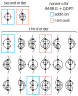
\includegraphics[width=.48\textwidth]{fig-diagrams-sfe}
\caption{Diagrammatic form of the second- and third-order QDPT corrections.  The diagrams are implicitly antisymmetrized (Hugenholtz diagrams), but also have implicit denominators as with many-body perturbation theory.}
\label{fig:diagrams-sfe}
\end{figure}

Since for this paper we are interested in the addition and removal energies, which involve one particle more or one particle less than a closed-shell state, we can take the label $u$ to be simply the label of the state that is added or removed from the closed-shell state $\Phi$.  With this realization, we can then express the perturbation expansion in terms of summations over matrix elements as we had done before for the IM-SRG flow equation, perhaps with the aid of Wick's theorem or diagrammatic techniques.  This leads to the following expression for the second-order correction:
\begin{align*}
  \epsilon_p^{(2)}
  &=
  \frac{1}{2} \sum_{i a b} \frac{n_i \bar{n}_a \bar{n}_b |H^{[2]}_{p i a b}|^2}{H^{[1]}_p + H^{[1]}_i - H^{[1]}_a - H^{[1]}_b} \\
  &{}-
  \frac{1}{2} \sum_{i j a} \frac{n_i n_j \bar{n}_a |H^{[2]}_{i j p a}|^2}{H^{[1]}_i + H^{[1]}_j - H^{[1]}_p - H^{[1]}_a}
\end{align*}
[[write out the full thing using $H^1_{p,p}$]]
The expression is depicted in Figure \ref{fig:diagrams-sfe}.  Since there are numerous terms in the third-order correction $\epsilon_p^{(3)}$, they are listed exclusively in a diagrammatic form in Figure \ref{fig:diagrams-sfe}.

Taking into account the perturbation corrections, one can obtain reasonably accurate addition and removal energies for single-particle states near the Fermi level via:
\begin{align*}
  \epsilon_p = H^{[1]}_{p, p} + \epsilon_p^{(2)} + \epsilon_p^{(3)}
\end{align*}

\subsection{Equations of Motion Methods}

Particle attached and particle removed equations of motion (EOM) methods can be coupled with either IM-SRG or coupled cluster calculations. The principal idea is that one may construct a ladder operator $\hat{X}$ that promotes the $N$-particle ground state to any state in the $N + 1$ or $N - 1$ spectrum,
\begin{equation}\label{eq:ladder_def}
  \ket{\Psi^{(N \pm 1)}_u}  = \hat{X}^{(N \pm 1)}_u \ket{\Psi^{(N)}_0},
\end{equation}
where $\hat{X}$ is in principle a linear combination of excitation and de-excitation operators that change particle number by one,
\begin{align}
  \label{eq:gen_attached}
  \hat{X}^{(N+1)}_u &= \sum_p \bar{n}_p x^{[1,0]}_p  \hat{a}^\dagger_p + \frac{1}{2} \sum^{[2,1]}_{p, q, r} \bar{n}_p \bar{n}_q n_r x_{p, q, r} \hat{a}^\dagger_p \hat{a}^\dagger_q \hat{a}_r + \cdots,  \\
  \label{eq:gen_removed}
  \hat{X}^{(N-1)}_u &= \sum_p n_p x_p^{[0,1]} \hat{a}_p + \frac{1}{2} \sum_{p, q, r} n_p n_q \bar{n}_r  x^{[1,2]}_{p, q, r} \hat{a}^\dagger_r \hat{a}_q \hat{a}_p  + \cdots.
\end{align}
Substitution of \eqref{eq:ladder_def} into the energy eigenvalue problem
\begin{gather*}
  \hat H \ket{\Psi_u^{(N \pm 1)}} = E^{(N\pm1)}_u \ket{\Psi_u^{(N \pm 1)}}
\end{gather*}
gives
\begin{equation}\label{eq:EOM}
  [\hat{H}, \hat{X}^{(N \pm 1)}_u] \ket{\Psi^{(N)}_0} = \pm \epsilon^{(\pm)}_u \hat{X}^{(N \pm 1)}_u \ket{\Psi^{(N)}_0},
\end{equation}
which constitutes a generalized eigenvalue problem for the amplitudes $x$, where $\epsilon^{(\pm)}_u$ are the single-particle addition ($+$) and removal ($-$) energies. The quality of this calculation depends on the ansatz for the $N$-particle ground state, as well as the systematically improvable truncation on the ladder operators. In this work we include 1p and 2p1h excitations in the $N + 1$ ladder operator and likewise 1h and 2h1p operators for the $N - 1$ ladder operators.

\subsubsection*{EOM-IM-SRG}
After a single-reference ground state IM-SRG calculation, the Hamiltonian has been rotated such that the reference state is an eigenfunction with corresponding eigenvalue $E^{(N)}_0$, which is the correlated $N$-particle ground state energy. The EOM equation is therefore
\begin{equation}\label{eq:EOMIMSRG}
  [\bar{H},\bar{X}^{(N \pm 1)}_u] \ket{\Phi^{(N)}_0} = \pm \epsilon^{(\pm)}_u \bar{X}^{(N \pm 1)}_u \ket{\Phi^{(N)}_0},
\end{equation}
where bars denote rotated operators. Now the reference state is used in place of the bare correlated ground state. The ground state IM-SRG procedure has implicitly re-summed contributions from higher order excitations (3-particle-2-hole, 2-particle-3-hole, 2-particle-3-hole, 4-particle-3-hole, \ldots) into the lower order amplitudes of the ladder operators (1-particle-0-hole, 0-particle-1-hole, 2-particle-1-hole, 1-particle-2-hole).

Despite these gains, the EOM calculation is still a partial diagonalization method, limited by the truncation to 2-particle-1-hole and 1-particle-2-hole operators. We expect $N + 1$ (or $N - 1$) states to be described appropriately by EOM-IM-SRG if their wavefunctions are dominated by 1-particle-0-hole (or 0-particle-1-hole) contributions in the rotated frame. We use partial norms of the EOM ladder operators to make this determination:
\begin{align}\label{eq:partial_norms}
  n_{\text{1-particle}} &= \sqrt{\sum_p \bar{n}_p | \bar{x}^{[1,0]}_p |^2},\\
  n_{\text{1-hole}} &= \sqrt{\sum_p n_p | \bar{x}^{[0,1]}_p |^2}.
\end{align}
Large single particle partial norms indicate that the EOM truncation is valid for the relevant state. States with lower single particle norms should be treated by with a higher EOM approximation, which can be accomplished directly or perturbatively. {\color{red} My paper talks about this a bit more, and we have some plots. Of course it only concerns the A-body stuff}.

\subsection{Diffusion Monte Carlo}
\label{subsec:DMC}

Diffusion Monte Carlo (DMC) is a method for calculating the ground state properties via a stochastic process akin to classical diffusion, refining an approximate ground state density towards that of the exact ground state.  The rules that govern the diffusion process are obtained by evolving the wave function using what can be formally be thought of as the time-dependent Schr\"odinger equation along imaginary time $\tau \equiv t / \mathrm{i}$:
\begin{align} \label{eq:itse}
  \frac{\partial}{\partial \tau} |\Phi(\tau)\rangle = \hat H |\Phi(\tau)\rangle
\end{align}
The solutions to this equation are not unlike the ordinary Schr\"odinger equation with a slight but crucial difference in the exponent:
\begin{align*}
  |\Phi(\tau)\rangle = \mathrm e^{-\hat H \tau} |\Phi(0)\rangle
\end{align*}
where $|\Phi(0)\rangle$ is the initial wave function at $\tau = 0$ -- not to be confused with the exact ground state of $\hat H$, which we denote $|\Psi_0\rangle$ here.  If we decompose the wave function into a sum over the eigenstates $|\Psi_n\rangle$,
\begin{align*}
  |\Psi(\tau)\rangle
  = \mathrm e^{-\hat H \tau} \sum_n c_n |\Psi_n\rangle
  = \sum_n c_n \mathrm e^{-E_n \tau} |\Psi_n\rangle
\end{align*}
we find that components of the wave function that have negative energy will increase exponentially as $\tau \to \infty$, while those with positive energy will decrease exponentially.  This property can be exploited to filter out the undesirable components, leaving only the ground state energy.  To do this, we require a trial energy $E_{\text{T}}$ -- a guess of the ground state energy -- and replace $\hat H$ in \eqref{eq:itse} with $(\hat H - E_{\text{T}})$ so that, if our trial energy is good, all states but the ground states will approximately vanish.

Diffusion Monte-Carlo (DMC) is a method used for refining a crude estimate to the ground state density into a better approximation to the exact ground state. The basic idea is to move multiple random walkers in position space with sampling rules which ensures convergence to a behavior representing a walk guided by the exact ground state density. Once a satisfying level of convergence is reached, expectation values are calculated by accumulating local estimates along the path of the walkers.

The equations representing the DMC algorithm is obtained by applying the projection operator $\hat{P}(\tau)$ on the crude trial state $\ket{\Psi_{\mathrm{T}}}$
\begin{equation}
 \hat{P}(\tau)\ket{\Psi_{\mathrm{T}}} \equiv \E^{-(\hat{H} - E_0)\tau} \ket{\Psi_{\mathrm{T}}}
\end{equation}
where $\tau$ is a constant often described as imaginary time, and $E_0=\bra{\Psi_0}\hat{H}\ket{\Psi_0}$ is the ground state of the Hamiltonian $\hat{H}$. By expanding the trial state in the eigenfunctions of $\hat{H}$, the ground state is obtained up to a constant factor
\begin{equation}
 \label{eq:DMC_ExactProjection}
 \lim_{\tau\to\infty} \bra{\bm{r}}  \hat{P}(\tau) \ket{\Psi_{\mathrm{T}}} = \braket{\Psi_0}{\Psi_{\mathrm{T}}}\Psi_0(\bm{r}).
\end{equation}

Defining $\Phi(\bm{r}, \tau) \equiv \bra{\bm{r}}\hat{P}(\tau)\ket{\Psi_{\mathrm{T}}}$, we obtain the state at a later time $\tau + \delta\tau$ through projection
\begin{align}
 \Phi(\bm{r}, \tau + \delta\tau) &= \bra{\bm{r}} P(\tau + \delta\tau) \ket{\Psi_{\mathrm{T}}} \notag\\
 &= \bra{\bm{r}} \E^{-(\hat{H} - E_0)\delta\tau} \hat{P}(\tau) \ket{\Psi_{\mathrm{T}}} \notag\\
 &= \bra{\bm{r}} \E^{-(\hat{H} - E_0)\delta\tau} \ket{\Phi(\tau)} \notag\\
 &= \int \D\bm{r}' \bra{\bm{r}} \E^{-(\hat{H} - E_0)\delta\tau} \ket{\bm{r}'} \Phi(\bm{r}', \tau)\notag \\
 &\equiv \int \D\bm{r}' G(\bm{r}, \bm{r}'; \delta\tau) \Phi(\bm{r}', \tau). \label{eq:DMC_GreenFuncRevealed}
\end{align}
which defines the Green's function $G$.

In practice, the ground state energy is a priori unknown, hence a trailing averaged value obtained from the converging DMC density is used. This energy is often referred to as the trial energy, and it is believed that with a sufficiently good trial state, the error due to this approximation is small.

The Green's function introduced in \eqref{eq:DMC_GreenFuncRevealed} has singularities due to the the Coulomb interaction term in $\hat{H}$. Due to Pauli exclusion these are not physical, nevertheless, in numerical implementations they are unpredictable and undesirable, hence we want to avoid them.

For evaluation of the local energy, the trial state is designed to cancel the Coulomb singularities by containing so-called correlation factors, however, this cancellation does not apply to the terms in the Green's function. In order to transfer this behavior to apply to the Green's function, a change to the formalism is introduced by iterating on a mixed density $f(\bm{r}, \tau) \equiv \Phi(\bm{r}, \tau)\Psi_{\mathrm{T}}(\bm{r})$. Note that all previous arguments regarding convergence to the true ground state still applies for the new distribution.

Methods exist for transforming the mixed density into the pure density $|\Phi(\bm{r}, \tau)|^2$ \cite{abInitioMC}, but unless the pure density is explicitly needed (e.g.~for comparisons with other methods), this is strictly not necessary.

Additionally, to avoid issues regarding the positive definiteness of the mixed distribution, the nodes of the mixed density is fixed to those of the wave function of the trial state. This is known as the \textit{fixed node approximation} \cite{umrigar:2865, abInitioMC}. Again, given a sufficiently good trial state, the errors should be small.

The Green's function for the mixed density is given as \cite{umrigar:2865}

\begin{align}
  G(\bm{r}, \bm{r}'; \delta\tau)_f &= \bra{\bm{r}} \E^{\frac{1}{2} \hat{\bm{\nabla}} \cdot \left(\hat{\bm{\nabla}} - \bm{F}(\bm{r})\right) - \left(E_{\mathrm{L}}(\bm{r}) - E_{\mathrm{T}}\right)} \ket{\bm{r}'} \label{eq:DMC_IS_GF_raw}\\
  &\propto \E^{-\left(|\bm{r} - \bm{r}' - \frac{1}{2}\delta\tau\bm{F}(\bm{r})|^2/(2\delta\tau)\right)} \label{eq:DMC_IS_GF}\\
  &\qquad\times \E^{-\left(\frac{1}{2}\left(E_{\mathrm{L}}(\bm{r'}) + E_{\mathrm{L}}(\bm{r})\right) - E_{\mathrm{T}}\right) \delta\tau} + \mathcal{O}\bigl((\delta\tau)^2\bigr), \notag
\end{align}
where
\begin{equation}
  \bm{F}(\bm{r}) = \frac{2 \hat{\bm{\nabla}} \Psi_{\mathrm{T}}(\bm{r})}{\Psi_{\mathrm{T}}(\bm{r})}
\end{equation}
is the drift vector commonly referred to as the \textit{quantum force}.

The local energy
\begin{equation}
E_{\mathrm{L}}(\bm{r}) \equiv \frac{\hat{H} \Psi_{\mathrm{T}}(\bm{r})}{\Psi_{\mathrm{T}}(\bm{r})}
\end{equation}
is necessarily sampled from $|\Psi_{\mathrm{T}}(\bm{r})|^2$ (ensured by using the Metropolis Algorithm \cite{abInitioMC}) to avoid undefined energies when sampling close to the nodes of $\Psi_{\mathrm{T}}(\bm{r})$.

The Green's function from \eqref{eq:DMC_IS_GF_raw} has been split into two for practical reasons; one part containing the kinetic terms, more specifically this represents a Fokker-Planck diffusion process, and a second part which is commonly referred to as a \textit{branching function}, which is an effective reweighing of a positions contribution to the overall density. Excluding branching we will simply sample from the density of the trial state.

In order dampen the errors introduced by splitting the Green's function, the time step $\delta\tau$ should be small. A value in the range of $10^{-3}$ to $10^{-4}$ is used in this work. High variance in energy samples requires a smaller time step to keep the branching controlled, since the fluctuations of the two are connected by \eqref{eq:DMC_IS_GF}.

The name branching arise from the fact that in DMC, the weights are implemented as a probability of a given walker to copy or delete itself $n$ times, where $\langle n \rangle$ equals the branching term of \eqref{eq:DMC_IS_GF}. Let $G_{\mathrm{b}}$ denote the value of the branching function at a given position. Correct weighting is then ensured by guaranteeing $m = \max\{0, \lfloor G_{\mathrm{b}} \rfloor - 1\}$ branches\footnote{$\lfloor x \rfloor$ denotes the floor of $x$, namely the largest integer $n$ such that $n \le x$.} with a probability $G_{\mathrm{b}} - m$ of getting an additional branch.  A branch is an identical copy of the corresponding walker, with an identical past but with a different future. When the number of requested branches is zero, the walker is removed from the simulation.


Initially, $N_{\mathrm{w}}$ walkers are initialized to span $|\Psi_{\mathrm{T}}(\bm{r})|^2$. This is ensured by using the Metropolis Algorithm. Moreover, importance sampling is ensured by sampling according to the kinetic term of \eqref{eq:DMC_IS_GF_raw} [[cite solution langevin]]

\begin{equation}
x_{i+1} = x_i + \frac{1}{2} \delta \tau F(\bm{r})_x + \xi,
\end{equation}
where $\xi$ is a uniform distributed random number with variance $\operatorname{Var}(\xi) = 2D\delta\tau$. A typical value of $N_{\mathrm{w}}$ in this work is \num{250000}.

For each time step, diffusion and branching repeats a given number of blocks $N_{\mathrm{b}}$ for each walker. New branches are not active until the next time step, and if a walker hits zero branches the block repetition stops. During these block loops, the trial energy $E_{\mathrm{T}}$ is sampled for use in the next time step $k+1$
\begin{equation}
 E_{\mathrm{T}}^{k+1} = \frac{1}{M_k}\sum_{i=1}^{M_k} G_{\mathrm{b}}(\bm{r}^{(k)}_i)E_{\mathrm{L}}(\bm{r}^{(k)}_i),
\end{equation}
where $M_k$ is the total number of samples obtained in cycle $k$. For this work we have found a value of $N_{\mathrm{b}} = 100$ to be sufficient.

Several methods for estimating $E_0$ exist in the literature, one of which is simply an average of all $N_{\mathrm{c}}$ trial energies calculated after $N_{\mathrm{t}}$ thermalization cycles
\begin{equation}
 E_0 = \frac{1}{N_{\mathrm{c}}-N_{\mathrm{t}}} \sum_{k=N_{\mathrm{t}}}^{N_{\mathrm{c}}} E_{\mathrm{T}}^{(k)}.
\end{equation}
This is the relation we use in this work to obtain the DMC energies.

In this work, the trial state has been chosen to consist of a single Slater determinant [[cite]] together with a single variational parameter Pad\'e-Jastrow correlation function [[cite]].

The Slater determinant contains eigenstates $\phi_n(\bm{r})$ of the 2-dimensional harmonic oscillator
with a variational parameter $\alpha$ scaling the oscillator frequency $\omega$
such that $\omega\to\alpha\omega$ in all solutions:
\begin{equation}
 \phi_n(\bm{r}) = H_n(\sqrt{\alpha\omega}x)H_n(\sqrt{\alpha\omega}y)\E^{-\alpha\omega r^2}.
\end{equation}
where $H_n$ is the $n$th level Hermite polynomial.

The eigenstates are selected such that the $N$ lowest lying energy eigenstates are selected (counting spin-degeneracy). Due to the Hamiltonian being spin independent we may split the Slater determinant into two equal parts -
one for each spin level [[cite]]. The overall form of the trial state is as follows:
\begin{equation}
 \Psi_{\mathrm{T}}(\bm{r}) \equiv S(\bm{r}^\uparrow) S(\bm{r}^\downarrow) \prod_{i<j}^{N} J(r_{i,j}),
\end{equation}
with
\begin{equation}
 S(\bm{r}^s) \equiv \begin{vmatrix}
\phi_1(\bm{r}^s_1) & \phi_2(\bm{r}^s_1)& \cdots & \phi_{N/2}(\bm{r}^s_1) \\
\phi_1(\bm{r}^s_2) & \phi_2(\bm{r}^s_2)& \cdots & \phi_{N/2}(\bm{r}^s_2) \\
\vdots & \vdots& \ddots & \vdots \\
\phi_1(\bm{r}^s_{N/2}) & \phi_2(\bm{r}^s_{N/2})& \cdots & \phi_{N/2}(\bm{r}^s_{N/2}) \\
 \end{vmatrix},
\end{equation}
and
\begin{equation}
 J(r_{i, j}) \equiv \exp\left(\frac{r_{i, j}}{1 + \beta r_{i, j}}\right),
\end{equation}
where $\bm{r}^s_i$ denotes $i$'th particle with spin $s$, and $r_{ij}$ is the relative distance between two electrons.
Since Metropolis Monte-Carlo only involves ratios of density functions, all normalization factors are skipped.

As a consequence of the variational principle, the optimal numeric values for $\alpha$ and $\beta$ can be found by minimizing the energy in the variational parameter space.  For this we have used the adaptive step gradient descent method [[cite ASGD]].

Using a single Slater determinant and a single variational parameter in the correlation function might at first glance seem insufficient,
however, the strength and robustness of DMC greatly succeeds at transforming this naive approximation into a very good estimate to the ground
state density. It should be mentioned that for systems where the single-particle Hamiltonian does not have analytical solutions, this approach
will indeed be insufficient due to low overlap between the initial and exact state.

A single Slater determinant and a simple correlation function opens up numerous optimization schemes which trivializes the computation time of most calculations.  We refer to Refs [[cite optimization techniques]] for more information.  Moreover, the most costly part of evaluating the single-particle eigenstates, the exponentials, is independent of the quantum number $n$, and can thus be tabulated once for the entire calculation. This holds for the gradient and Laplacian needed in the quantum force and local energy, respectively, since the exponential shape is preserved under differentiation.

\section{Results}
\label{sec:results}

\begin{figure}
  \centering
  \subfigure[Results for $N=6$ and $\omega=1.0$]{
    \label{fig:N6hw1}
    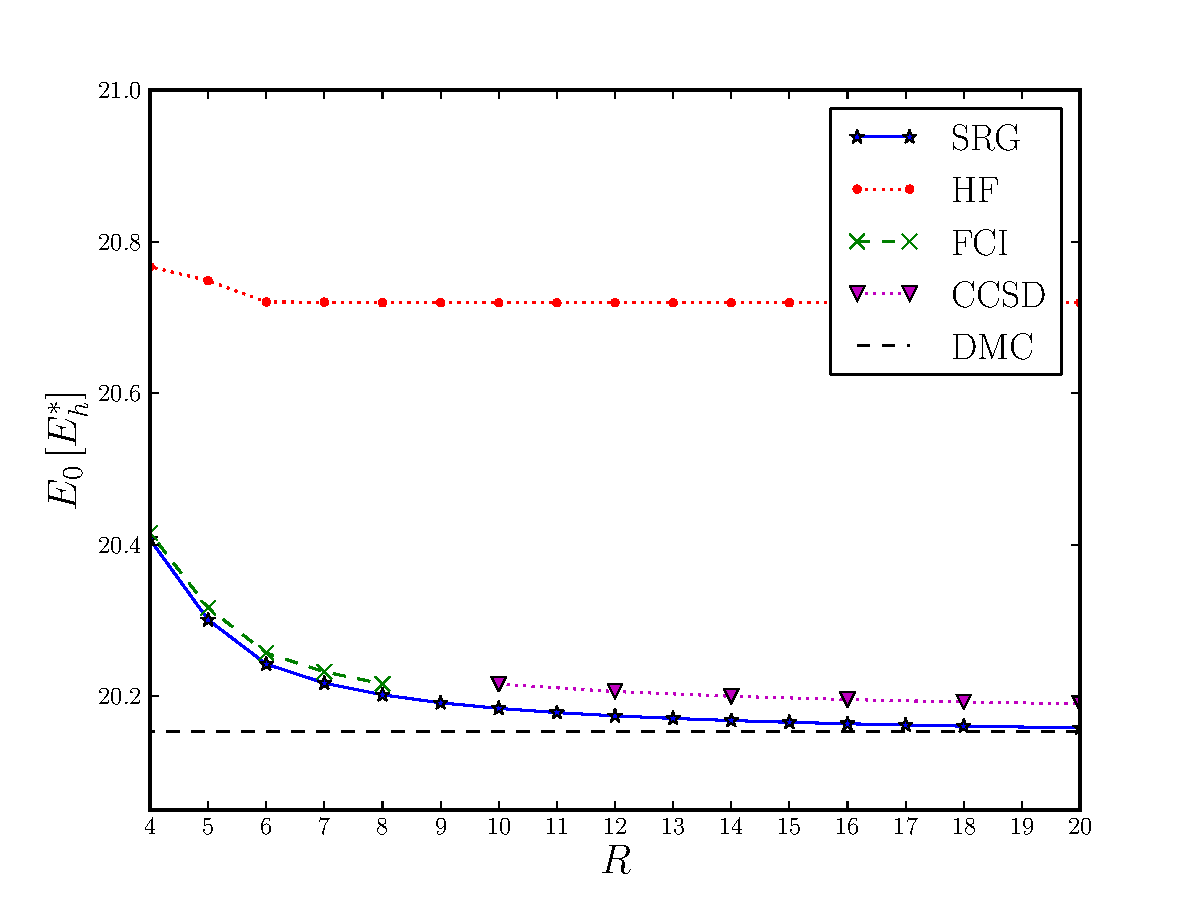
\includegraphics[width=0.38\textwidth]{figures/6parthw1.pdf}
  }
  \subfigure[Results for $N=6$ and $\omega=0.5$]{
    \label{fig:N6hw05}
    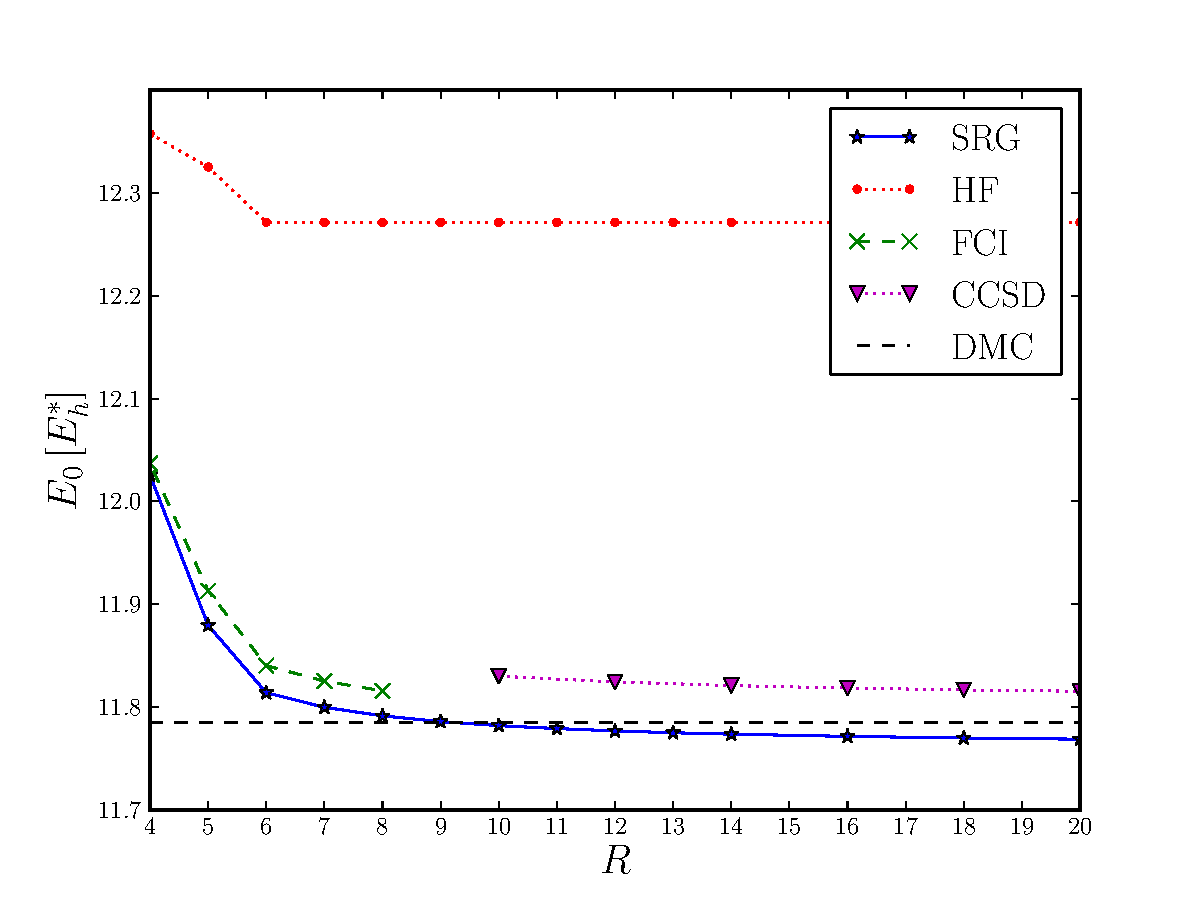
\includegraphics[width=0.38\textwidth]{figures/6parthw05.pdf}
  } \\
  \subfigure[Results for $N=6$ and $\omega=0.28$]{
    \label{fig:N6hw028}
    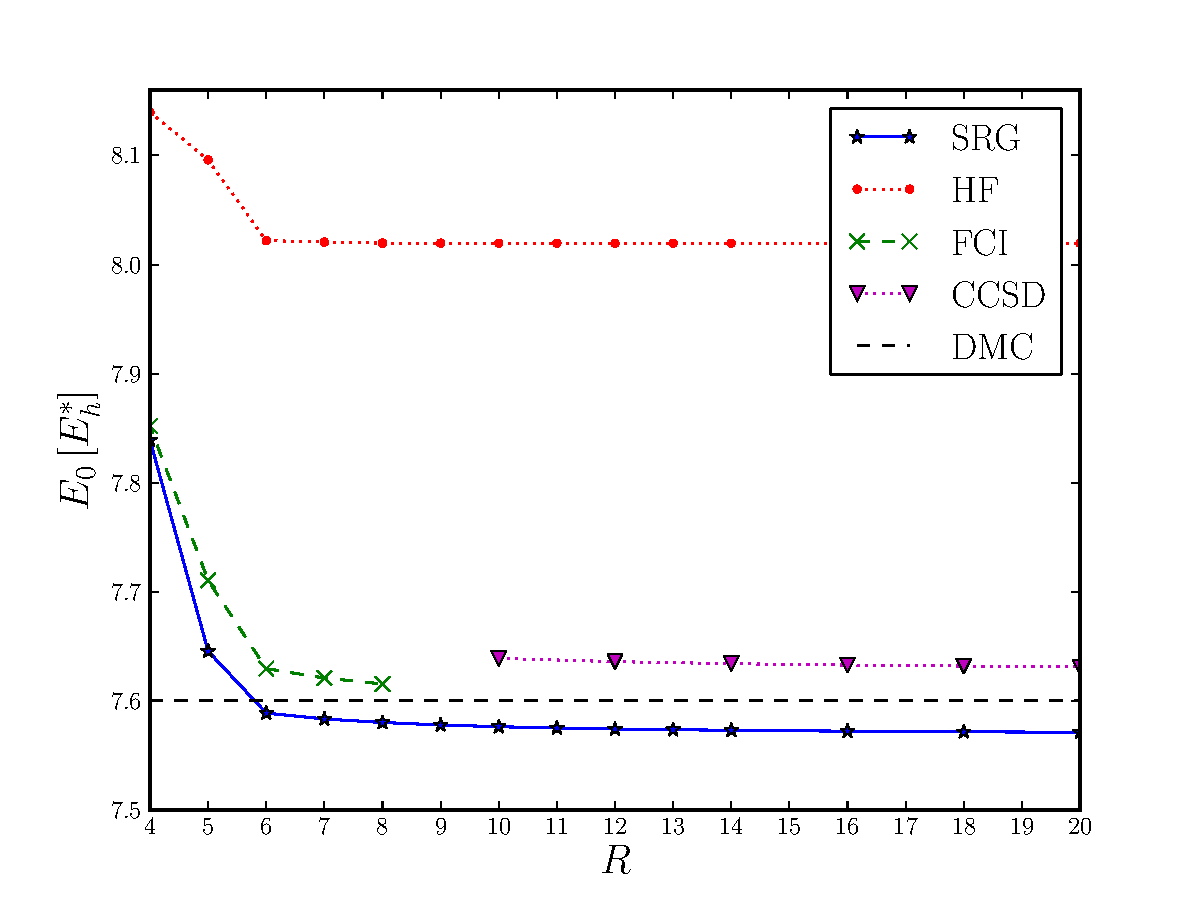
\includegraphics[width=0.38\textwidth]{figures/6parthw028.pdf}
  }
  \subfigure[Results for $N=6$ and $\omega=0.1$]{
    \label{fig:N6hw01}
    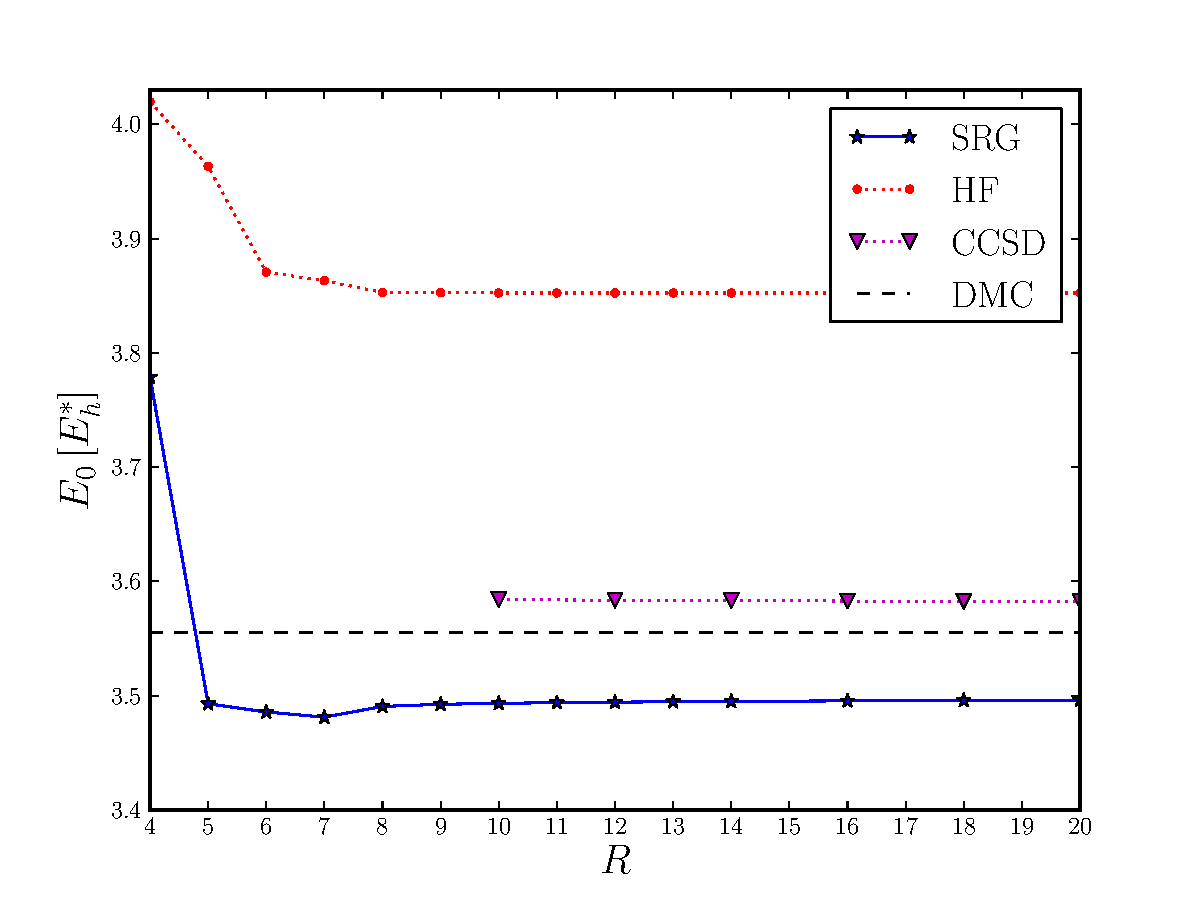
\includegraphics[width=0.38\textwidth]{figures/6parthw01.pdf}
  }
  \caption{Comparison of our IM-SRG(2) ground state energies (SRG) for circular quantum dots for $N=6$ and $\omega=1.0$ The results are compared with diffusion Monte Carlo (DMC), coupled cluster at the level of singles and doubles (CCSD), full configuration interaction (FCI) and Hartree-Fock calculations (HF) as functions of the number of major oscillator shells $R$. A harmonic oscilaltor basis has been used, with an unrenormalized Coulomb repulsion and the White generator. All energies in atomic units.}
  \label{fig:N6}
\end{figure}

\begin{figure}
  \centering
  \subfigure[Results for $N=12$ and $\omega=1.0$]{
    \label{fig:N12hw1}
    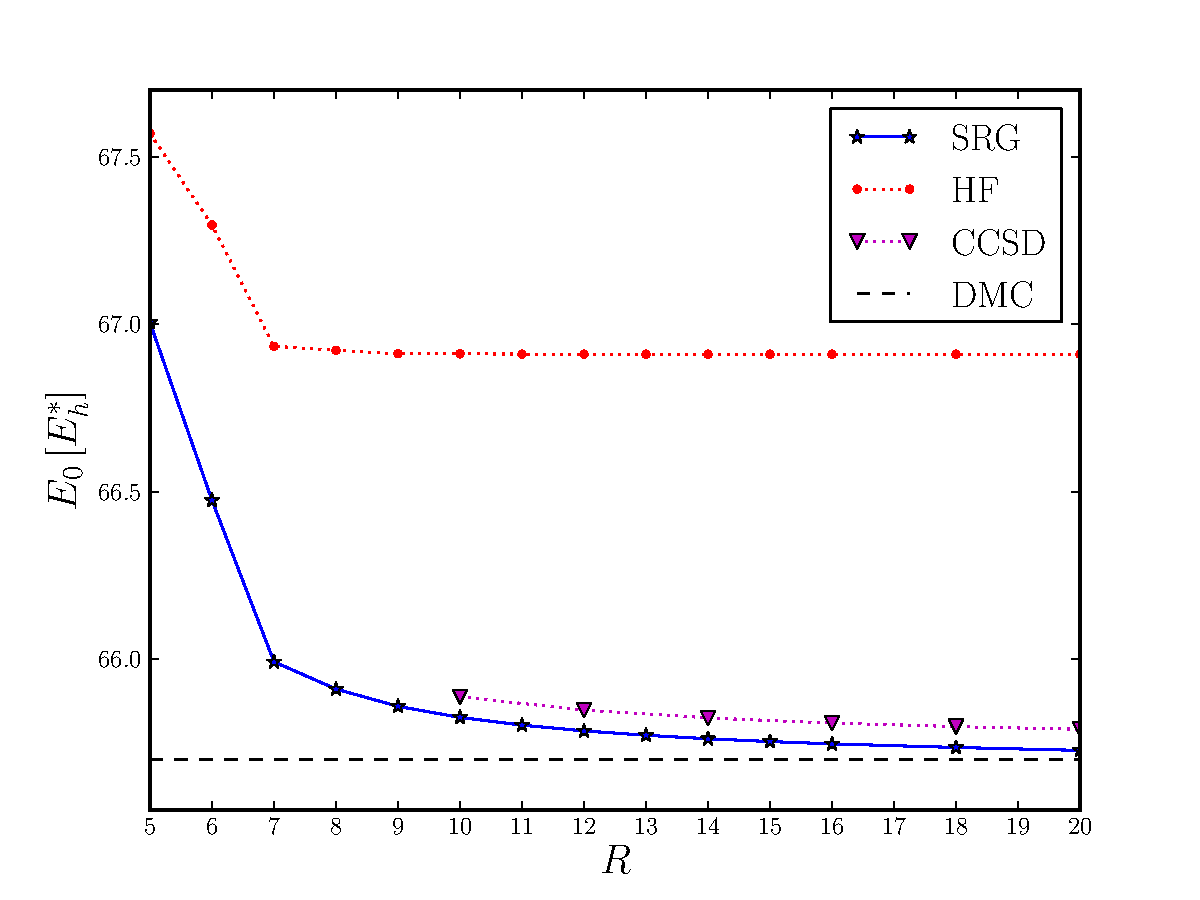
\includegraphics[width=0.38\textwidth]{figures/12parthw1.pdf}
  }
  \subfigure[Results for $N=12$ and $\omega=0.5$]{
    \label{fig:N12hw05}
    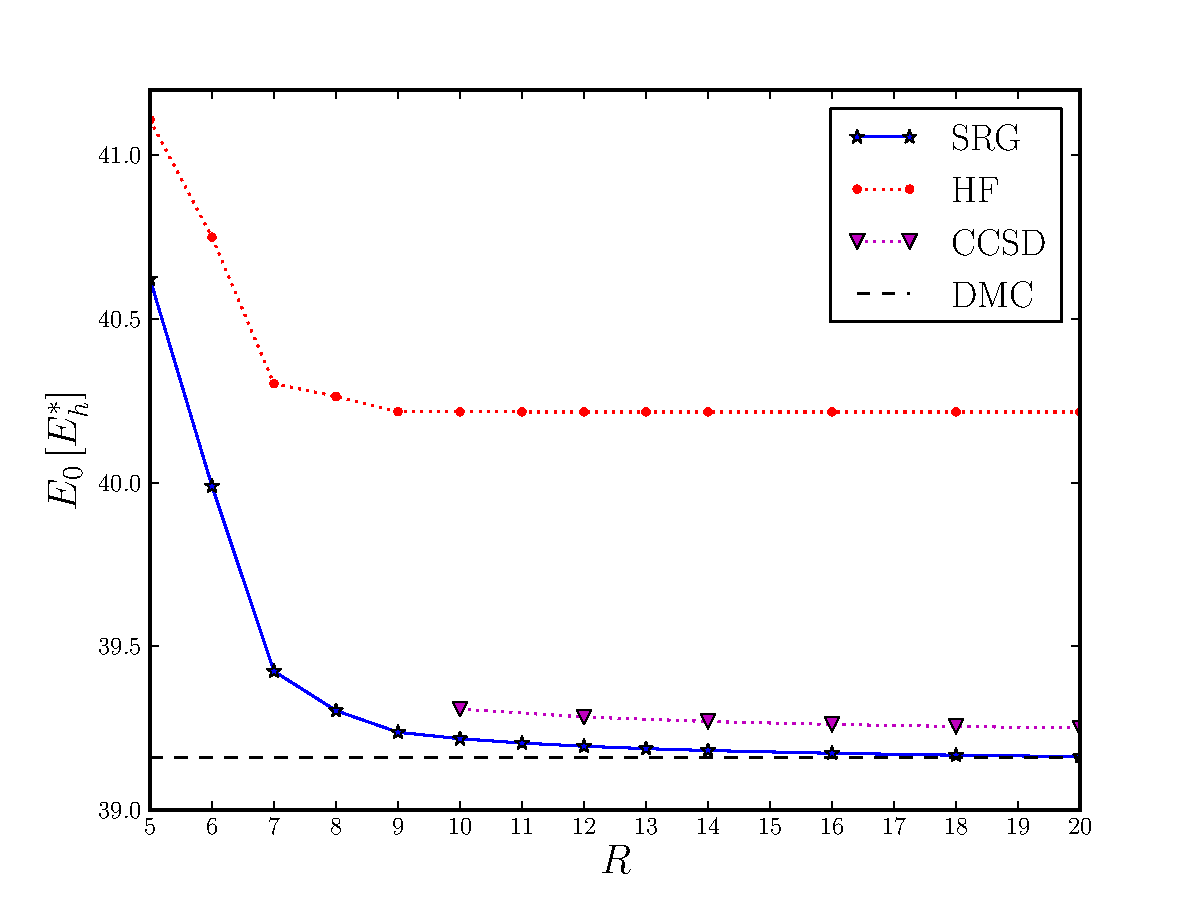
\includegraphics[width=0.38\textwidth]{figures/12parthw05.pdf}
  } \\
  \subfigure[Results for $N=12$ and $\omega=0.28$]{
    \label{fig:N12hw028}
    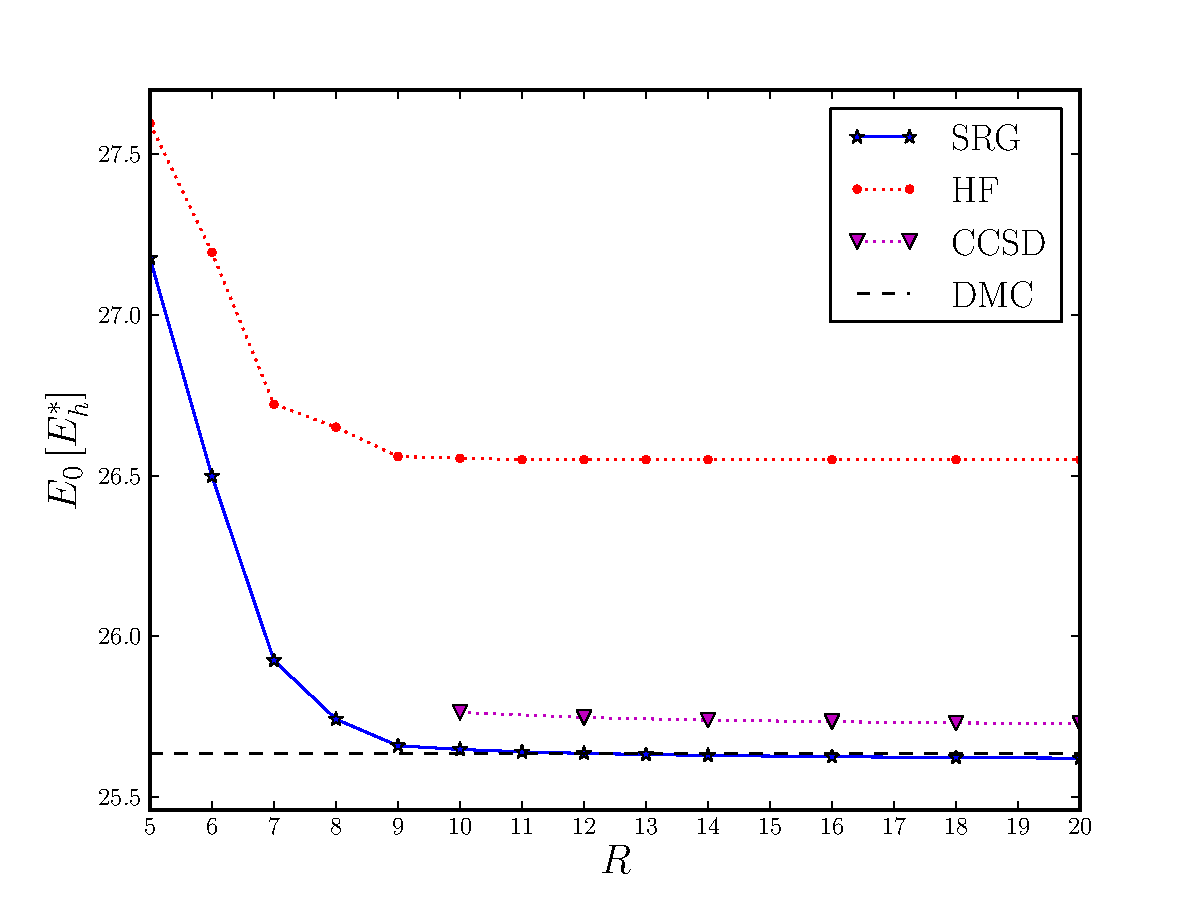
\includegraphics[width=0.38\textwidth]{figures/12parthw028.pdf}
  }
  \subfigure[Results for $N=12$ and $\omega=0.1$]{
    \label{fig:N12hw01}
    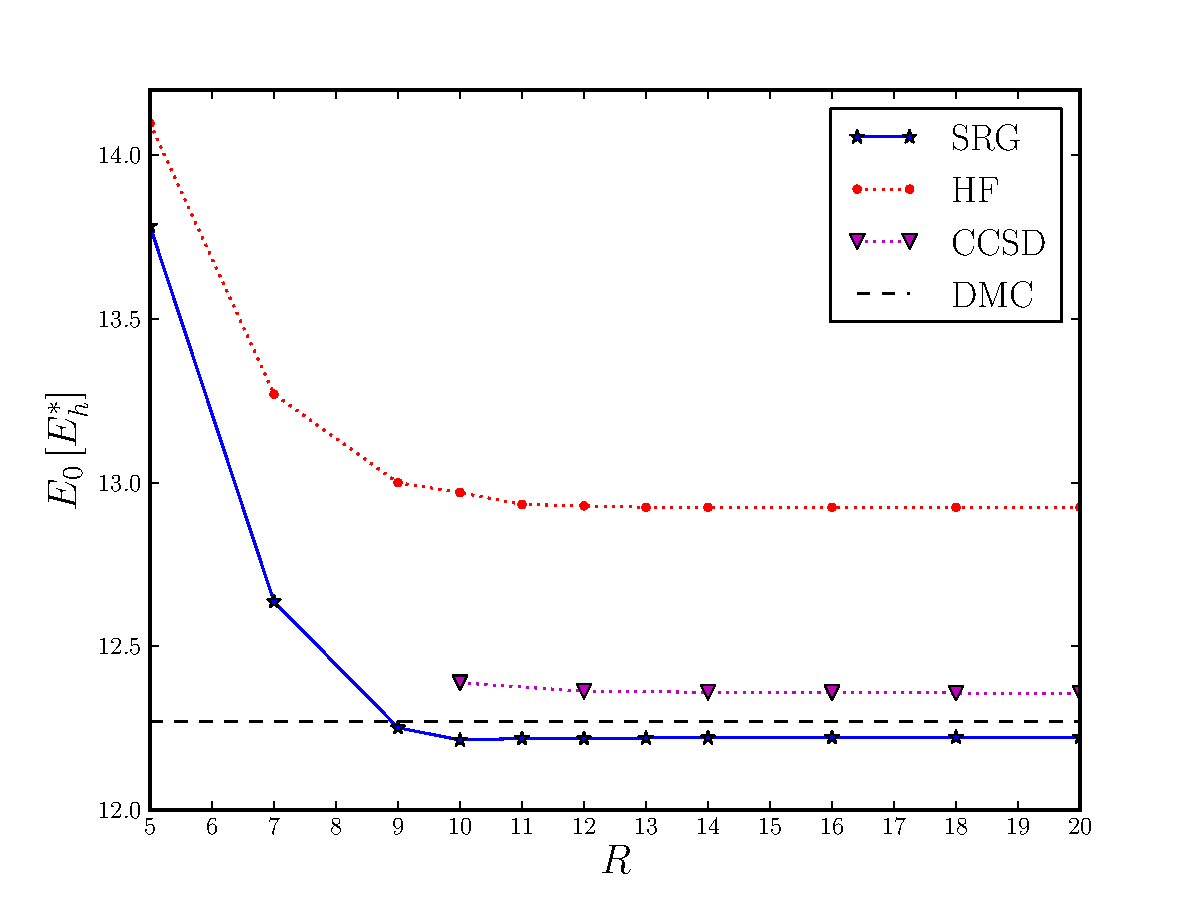
\includegraphics[width=0.38\textwidth]{figures/12parthw01.pdf}
  }
  \caption{Comparison of our IM-SRG(2) ground state energies (SRG) for circular quantum dots for $N=12$ and different values of $\omega$. The results are compared with diffusion Monte Carlo (DMC), coupled cluster at the level of singles and doubles (CCSD), full configuration interaction (FCI) and Hartree-Fock calculations (HF) as functions of the number of major oscillator shells $R$. A harmonic oscilaltor basis has been used, with an unrenormalized Coulomb repulsion and the White generator. All energies in atomic units.}
  \label{fig:N12}
\end{figure}

\begin{figure}
  \centering
  \subfigure[Results for $N=20$ and $\omega=1.0$]{
    \label{fig:N20hw1}
    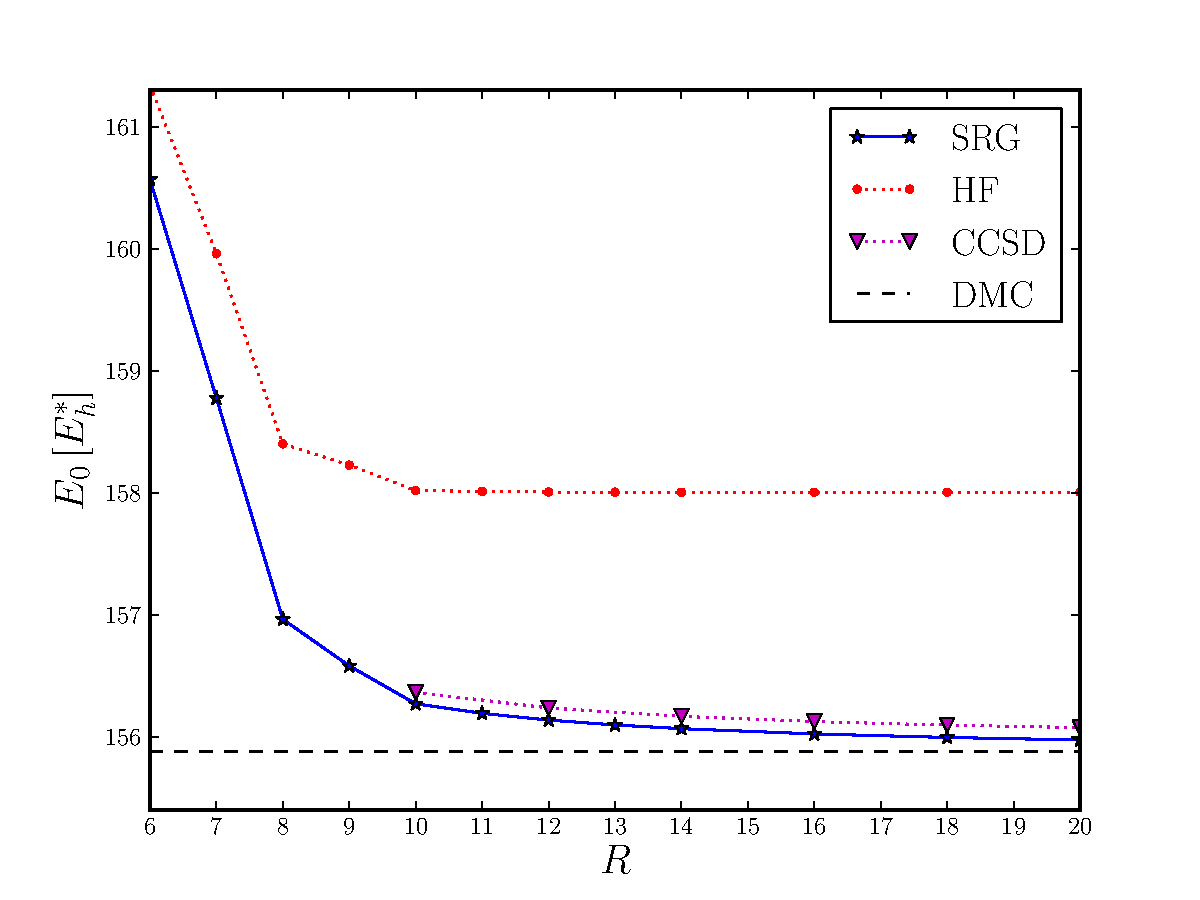
\includegraphics[width=0.38\textwidth]{figures/20parthw1.pdf}
  } \subfigure[Results for $N=20$ and $\omega=0.5$]{
    \label{fig:N20hw05}
    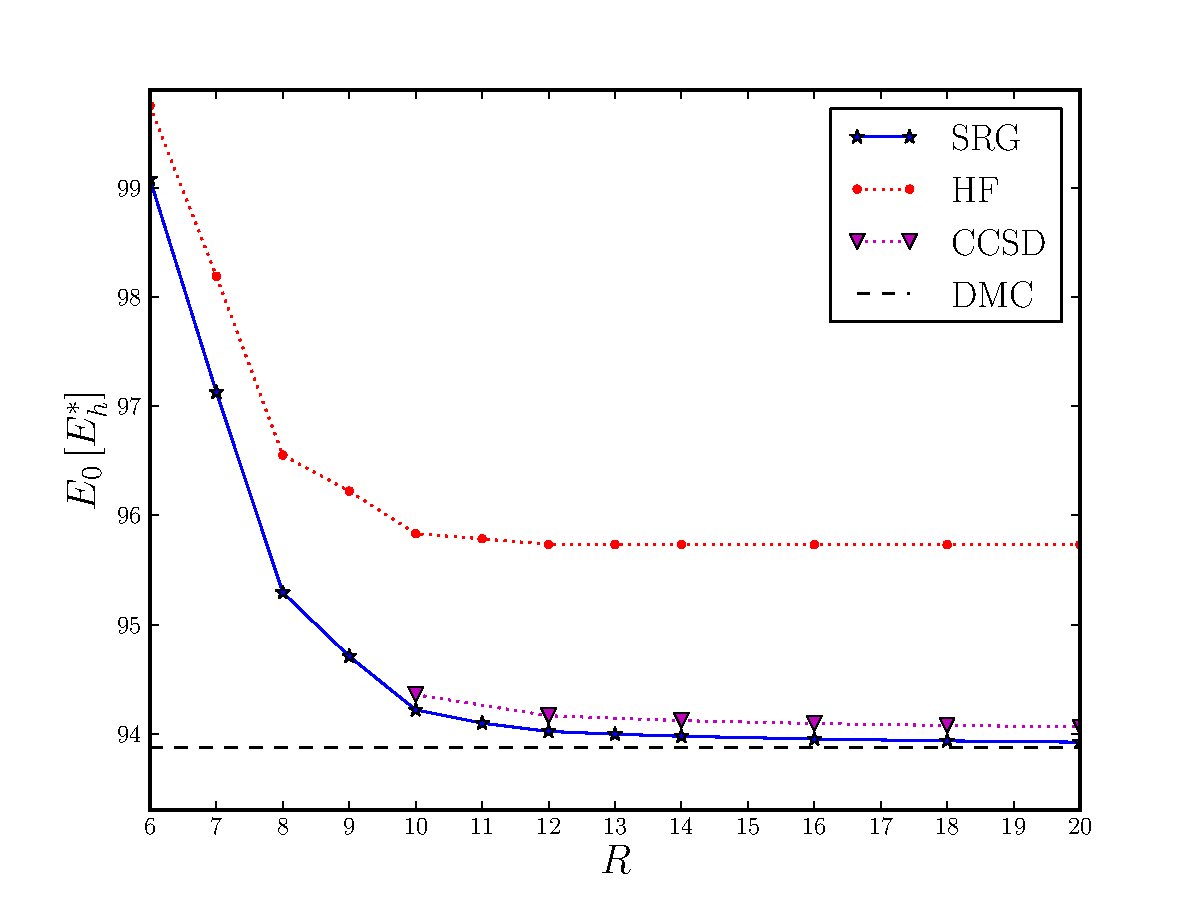
\includegraphics[width=0.38\textwidth]{figures/20parthw05.pdf}
  } \\
  \subfigure[Results for $N=20$ and $\omega=0.28$]{
    \label{fig:N20hw028}
    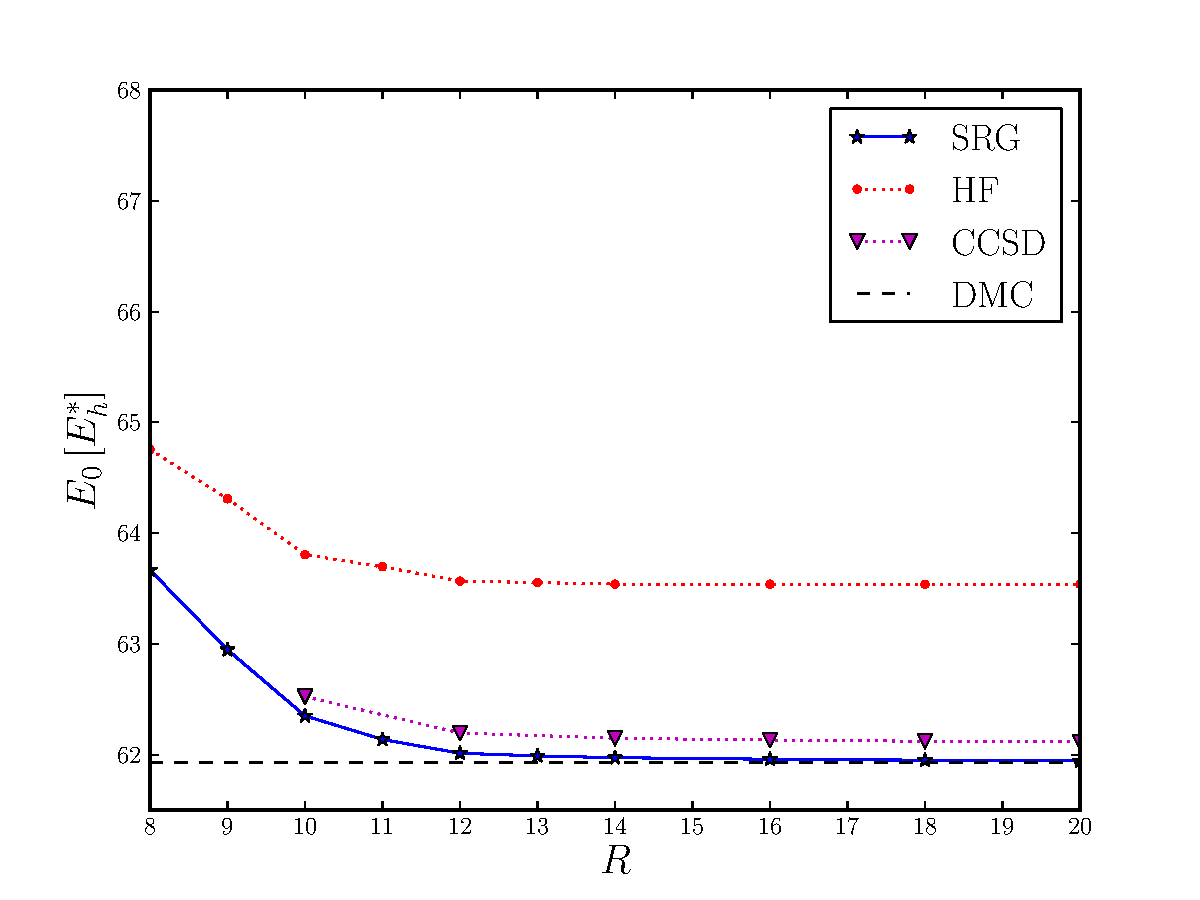
\includegraphics[width=0.38\textwidth]{figures/20parthw028.pdf}
  } \subfigure[Results for $N=20$ and $\omega=0.1$]{
    \label{fig:N20hw01}
    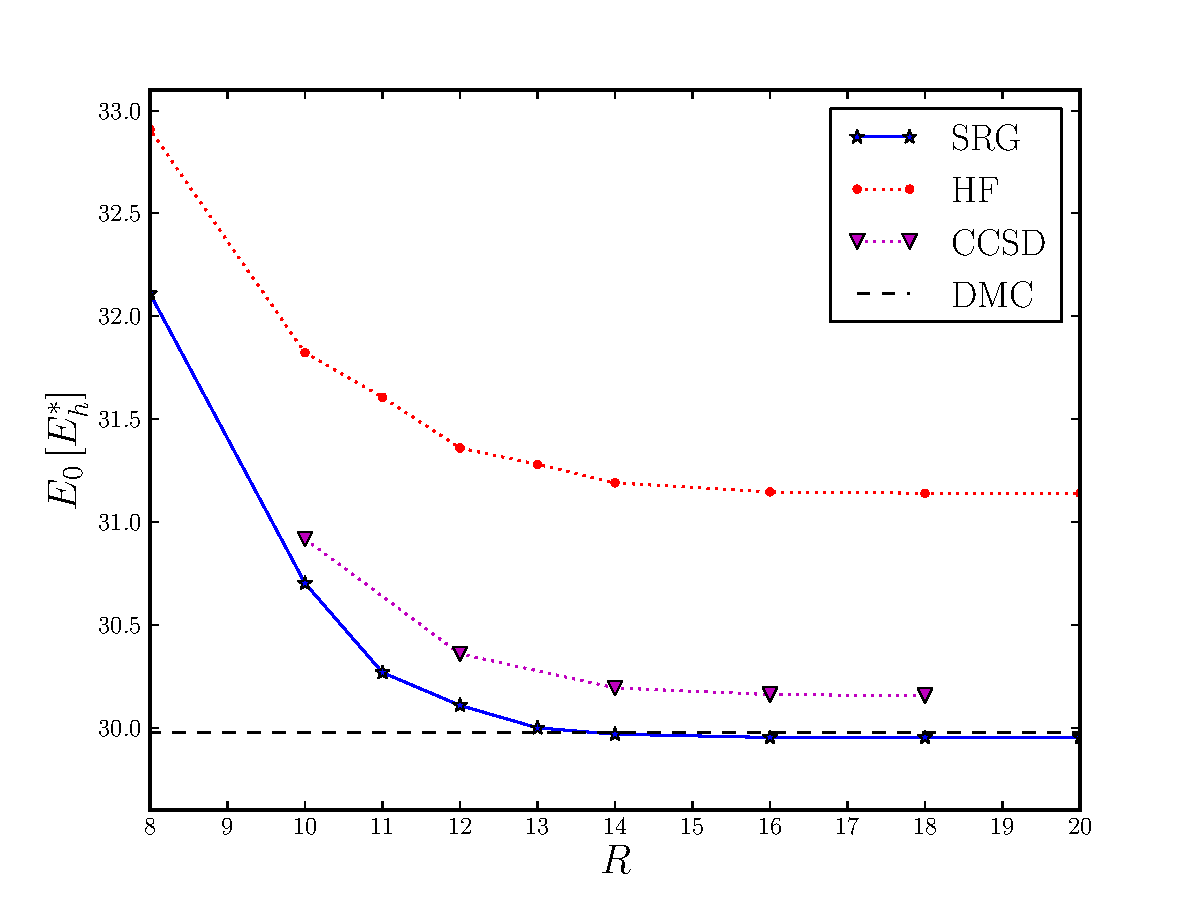
\includegraphics[width=0.38\textwidth]{figures/20parthw01.pdf}
  }
  \caption{Comparison of our IM-SRG(2) ground state energies (SRG)
    for circular quantum dots for $N=20$ and different values of
    $\omega$. The results are compared with diffusion Monte
    Carlo (DMC), coupled cluster at the level of singles and doubles
    (CCSD), full configuration interaction (FCI) and Hartree-Fock
    calculations (HF) as functions of the number of major oscillator
    shells $R$. A harmonic oscilaltor basis has been used, with an
    unrenormalized Coulomb repulsion and the White generator. All
    energies in atomic units.}
  \label{fig:N20}
\end{figure}

\begin{figure}
  \centering
  \subfigure[Results for $N=30$ and $\omega=1.0$]{
    \label{fig:N30hw1}
    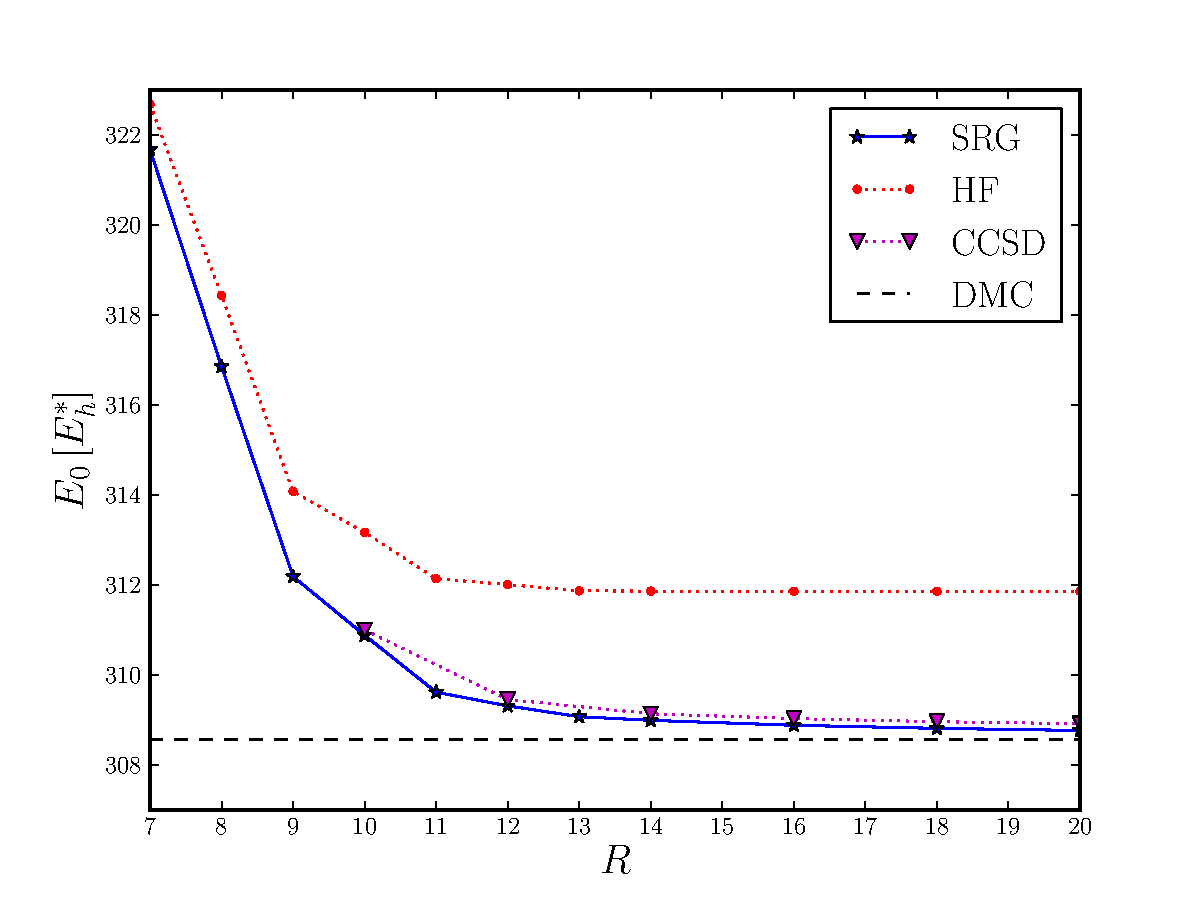
\includegraphics[width=0.38\textwidth]{figures/30parthw1.pdf}
  } \subfigure[Results for $N=30$ and $\omega=0.5$]{
    \label{fig:N30hw05}
    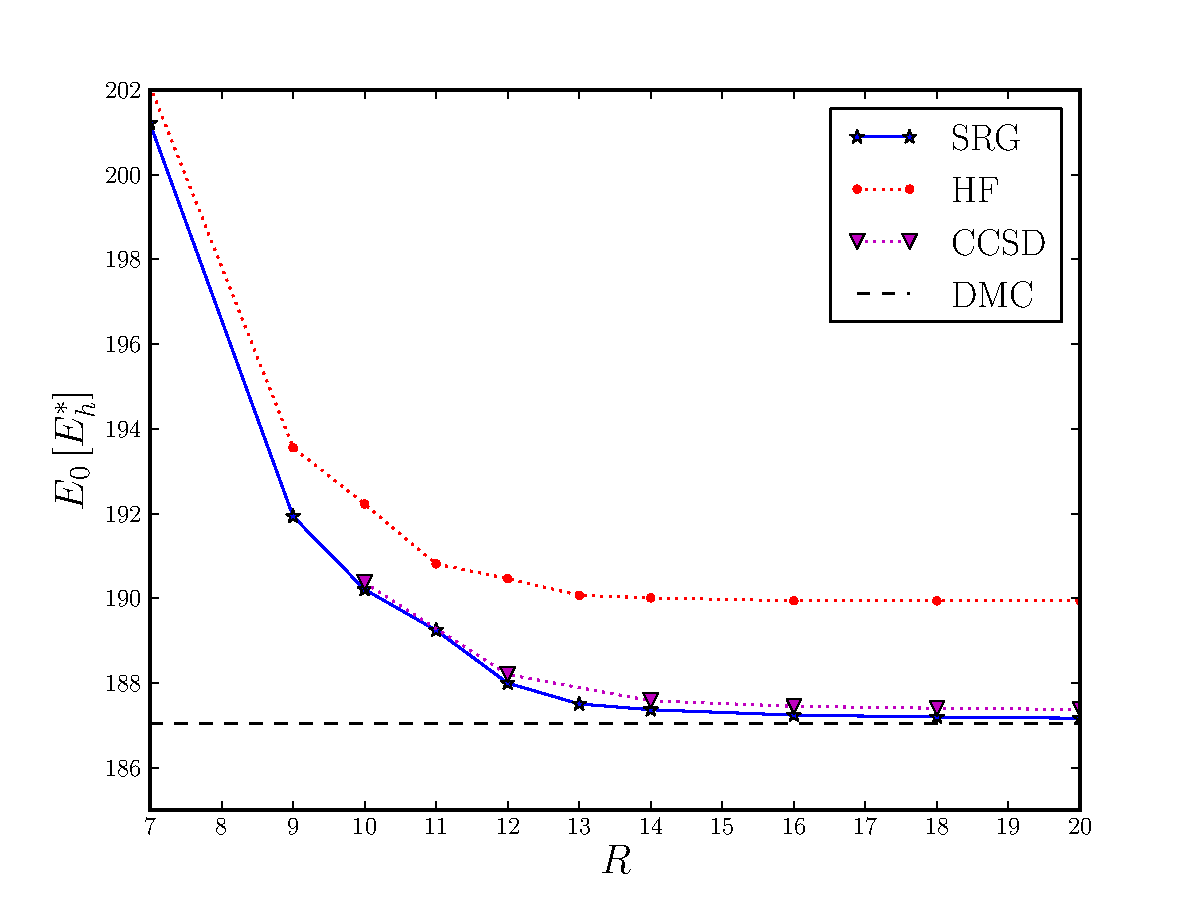
\includegraphics[width=0.38\textwidth]{figures/30parthw05.pdf}
  } \\
  \subfigure[Results for $N=30$ and $\omega=0.28$]{
    \label{fig:N30hw028}
    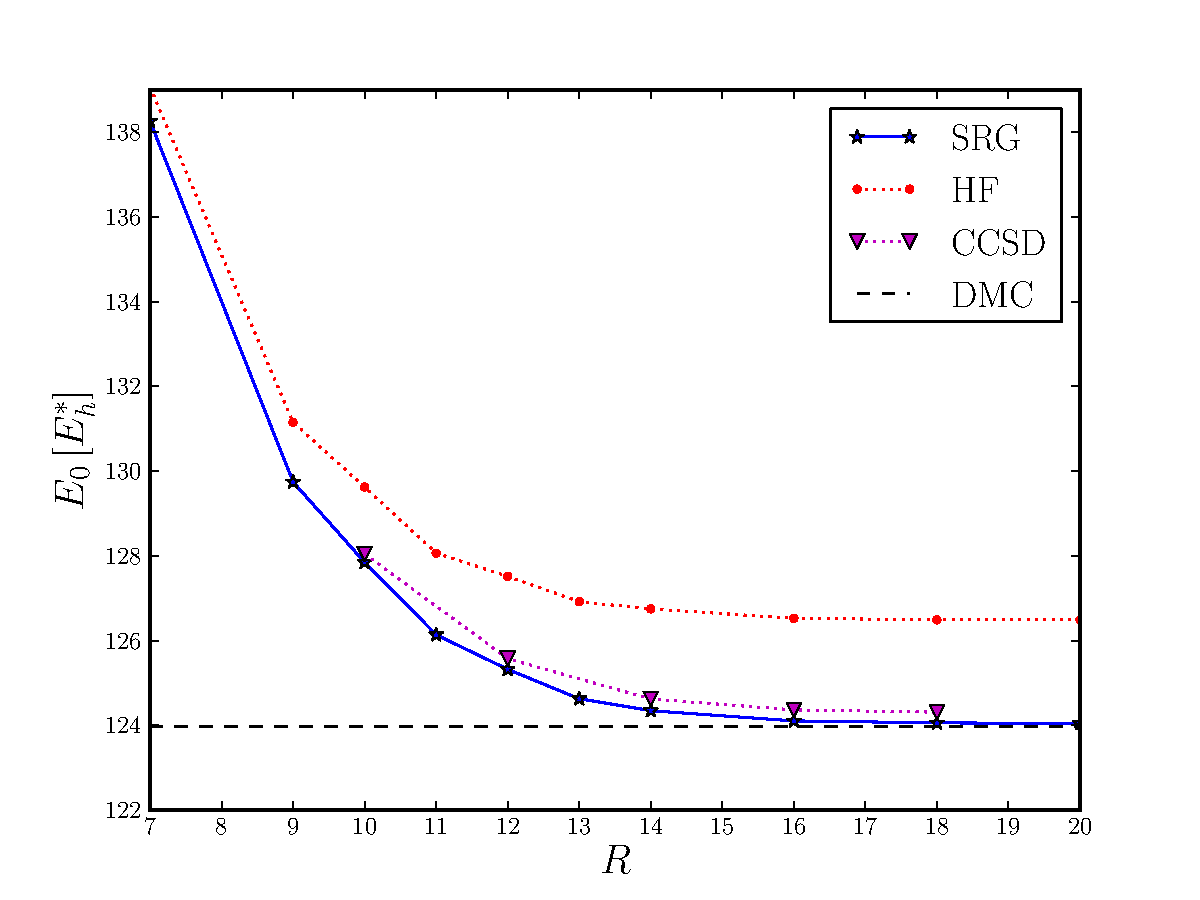
\includegraphics[width=0.38\textwidth]{figures/30parthw028.pdf}
  } \subfigure[Results for $N=30$ and $\omega=0.1$]{
    \label{fig:N30hw01}
    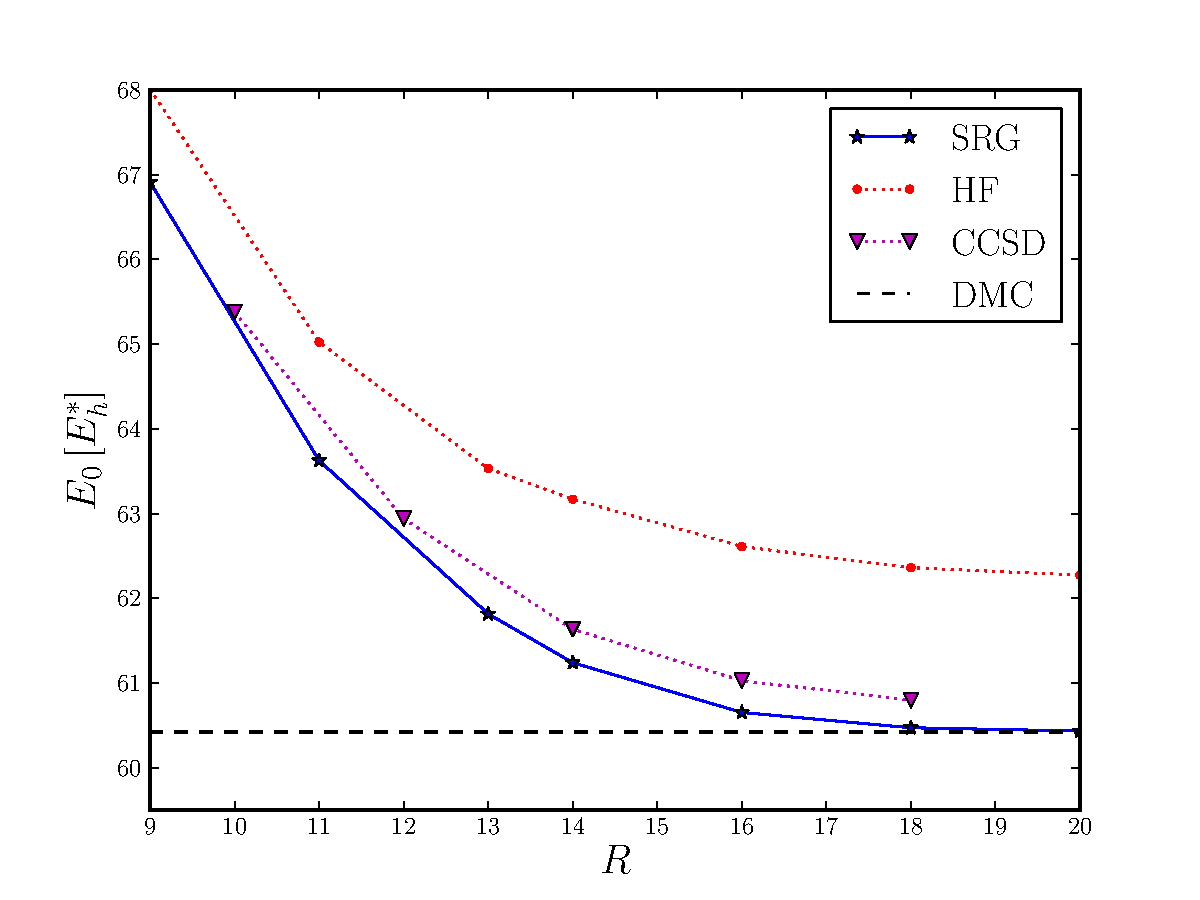
\includegraphics[width=0.38\textwidth]{figures/30parthw01.pdf}
  }
  \caption{Comparison of our IM-SRG(2) ground state energies (SRG)
    for circular quantum dots for $N=30$ and different values of
    $\omega$. The results are compared with diffusion Monte
    Carlo (DMC), coupled cluster at the level of singles and doubles
    (CCSD), full configuration interaction (FCI) and Hartree-Fock
    calculations (HF) as functions of the number of major oscillator
    shells $R$. A harmonic oscilaltor basis has been used, with an
    unrenormalized Coulomb repulsion and the White generator. All
    energies in atomic units.}
  \label{fig:N30}
\end{figure}

\begin{figure}
  \centering
  \subfigure[Results for $N=42$ and $\omega=1.0$]{
    \label{fig:N42hw1}
    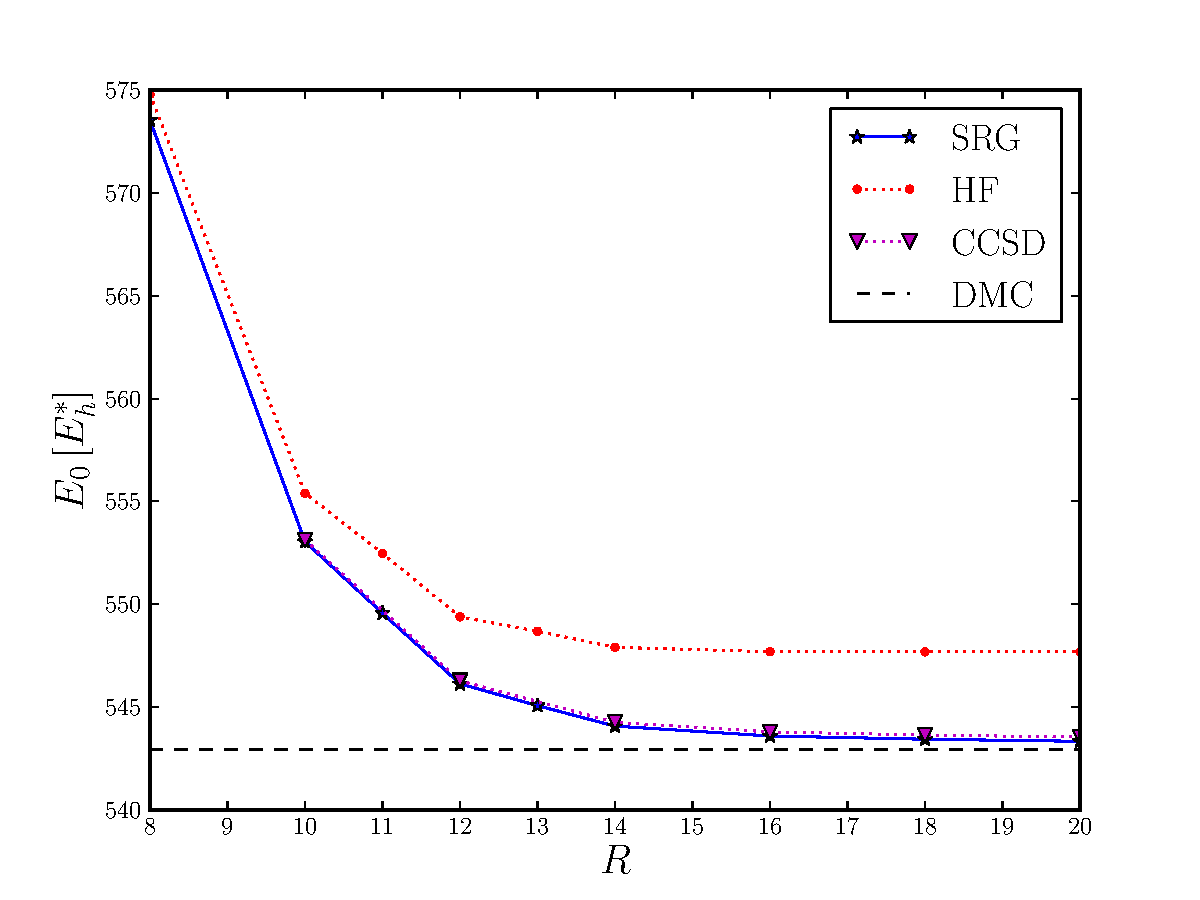
\includegraphics[width=0.38\textwidth]{figures/42parthw1.pdf}
  } \subfigure[Results for $N=42$ and $\omega=0.5$]{
    \label{fig:N42hw05}
    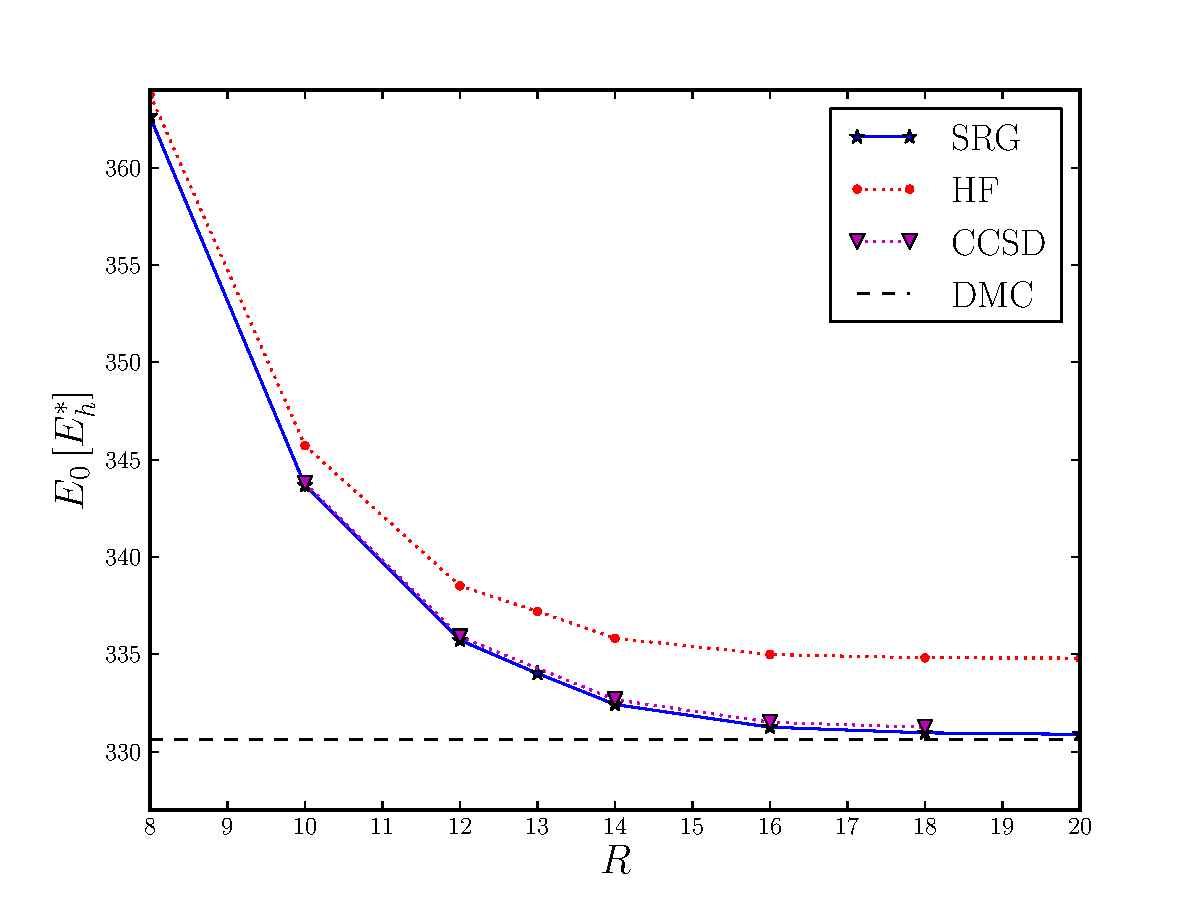
\includegraphics[width=0.38\textwidth]{figures/42parthw05.pdf}
  } \\
  \subfigure[Results for $N=42$ and $\omega=0.28$]{
    \label{fig:N42hw028}
    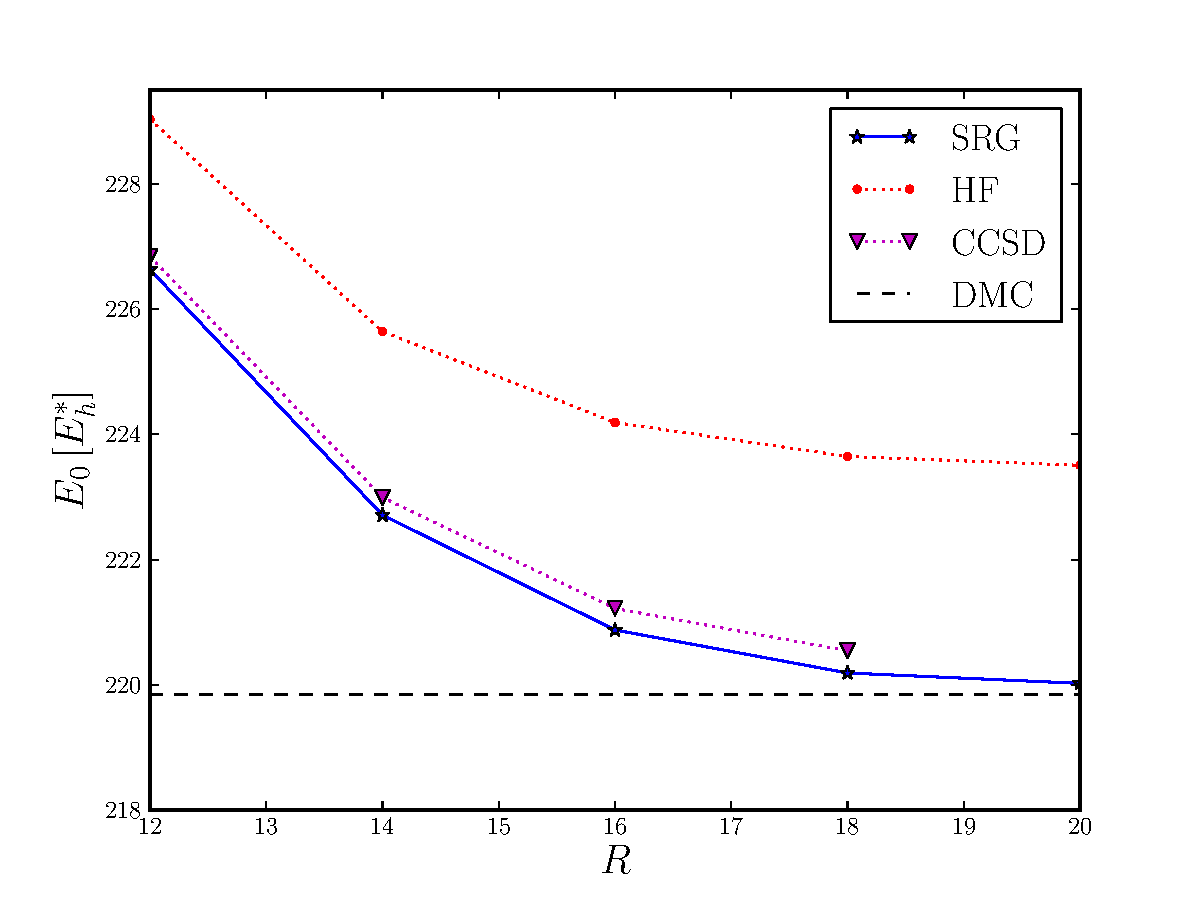
\includegraphics[width=0.38\textwidth]{figures/42parthw028.pdf}
  } \subfigure[Results for $N=42$ and $\omega=0.1$]{
    \label{fig:N42hw01}
    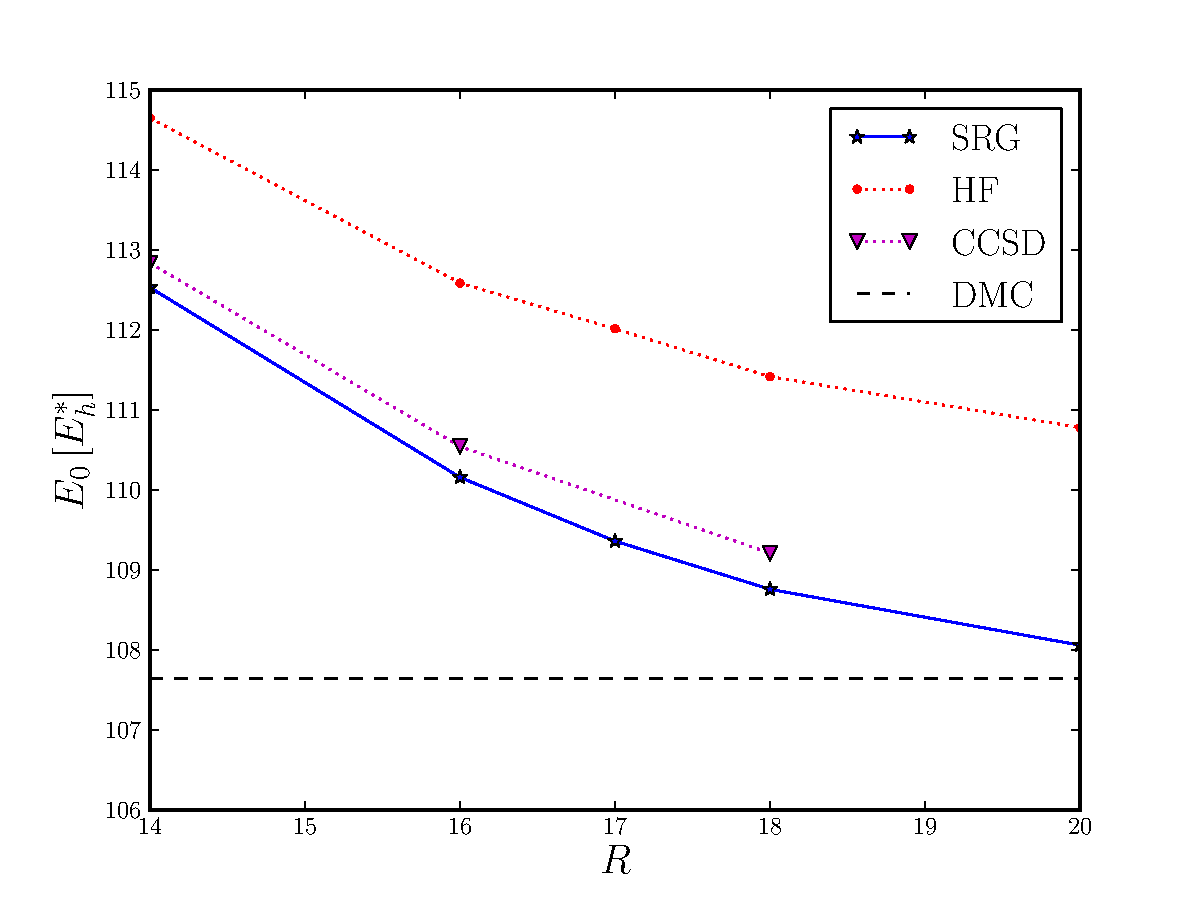
\includegraphics[width=0.38\textwidth]{figures/42parthw01.pdf}
  }
  \caption{Comparison of our IM-SRG(2) ground state energies (SRG) for circular quantum dots for $N=42$ and different values of $\omega$. The results are compared with diffusion Monte Carlo (DMC), coupled cluster at the level of singles and doubles (CCSD), full configuration interaction (FCI) and Hartree-Fock calculations (HF) as functions of the number of major oscillator shells $R$. A harmonic oscilaltor basis has been used, with an unrenormalized Coulomb repulsion and the White generator. All energies in atomic units.}
  \label{fig:N42}
\end{figure}

\begin{table}
  \centering
  \caption{Ground state energy (in atomic units) of a circular quantum dot, with $N$ particles and oscillator frequency $\omega$. The IM-SRG(2) results are given for $R=20$ shells (except for the $N=56$ results which are for $R=18$), employing a Hartree-Fock basis, a bare Coulomb interaction and the White generator. For $N=42$ and $\omega=0.1$ results are presented up to $R=22$ major shells. The results labelled IM-SRG(2)$_{R\rightarrow \infty}$ are obtained using the extrapolation formula of [[equation?]].}
  \label{tab:SRGDMC-R20}
  \begin{tabular}{SSSSS}
    \toprule
    {$N$} & {$\omega$} & {IM-SRG(2)} & {IM-SRG(2)$_{R\rightarrow \infty}$} & {DMC} \\
    \midrule
    6  & 1.0  &  20.1583  &  20.1468 &  20.1593(1) \\
       & 0.5  &  11.7690  &  11.7631 &  11.7848(1) \\
       & 0.28 &   7.5713  &   7.5695 &   7.6002(1) \\
       & 0.1  &   3.4962  &   3.4977 &   3.5539(1) \\
    \midrule
    12 & 1.0  &  65.7280  &  65.6990 &  65.7001(1) \\
       & 0.5  &  39.1631  &  39.1473 &  39.1596(1) \\
       & 0.28 &  25.6212  &  25.6140 &  25.6358(1) \\
       & 0.1  &  12.2223  &  12.2234 &  12.2698(1) \\
    \midrule
    20 & 1.0  & 155.9737  & 155.9130 & 155.8822(1) \\
       & 0.5  &  93.9219  &  93.8853 &  93.8752(1) \\
       & 0.28 &  61.94362 &  61.9240 &  61.9268(1) \\
       & 0.1  &  29.95263 &  29.9565 &  29.9779(1) \\
    \midrule
    30 & 1.0  & 308.7673  & 308.6053 & 308.5627(2) \\
       & 0.5  & 187.1671  & 186.8340 & 187.0426(2) \\
       & 0.28 & 124.0410  & 123.7171 & 123.9683(2) \\
       & 0.1  &  60.4319  &  60.1158 &  60.4205(2) \\
    \midrule
    42 & 1.0  & 543.3398  & 543.3304 & 542.9428(8) \\
       & 0.5  & 330.8885  & 330.8425 & 330.6306(2) \\
       & 0.28 & 220.0226  & 219.9534 & 219.8426(2) \\
       & 0.1  & 107.7851  & 106.8074 & 107.6389(2) \\
    \midrule
    56 & 1.0  & 880.4159  &          & 879.3986(6) \\
       & 0.5  & 538.8199  &          & 537.353(2)  \\
       & 0.28 & 360.83689 &          & 358.145(2)  \\
    \bottomrule
  \end{tabular}
\end{table}

\begin{figure}
  \centering
  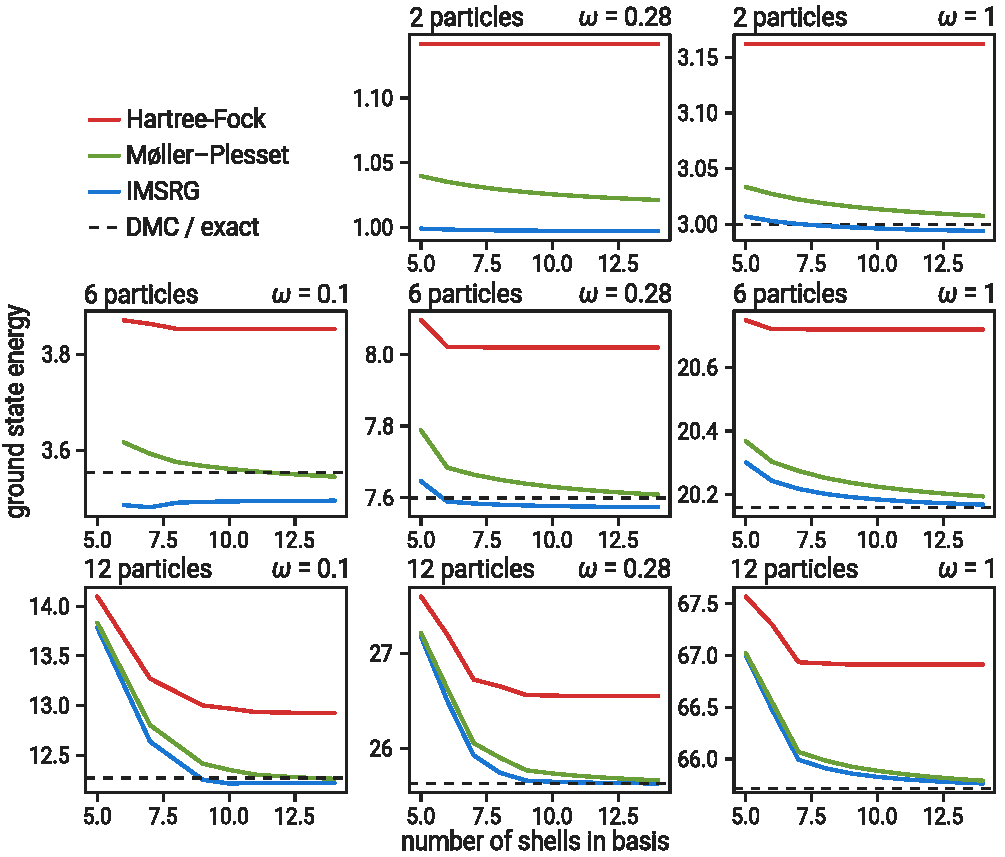
\includegraphics[width=0.8\textwidth]{fig-gs}
  \caption{Ground state energies.}
  \label{fig:gs}
\end{figure}

\begin{figure}
  \centering
  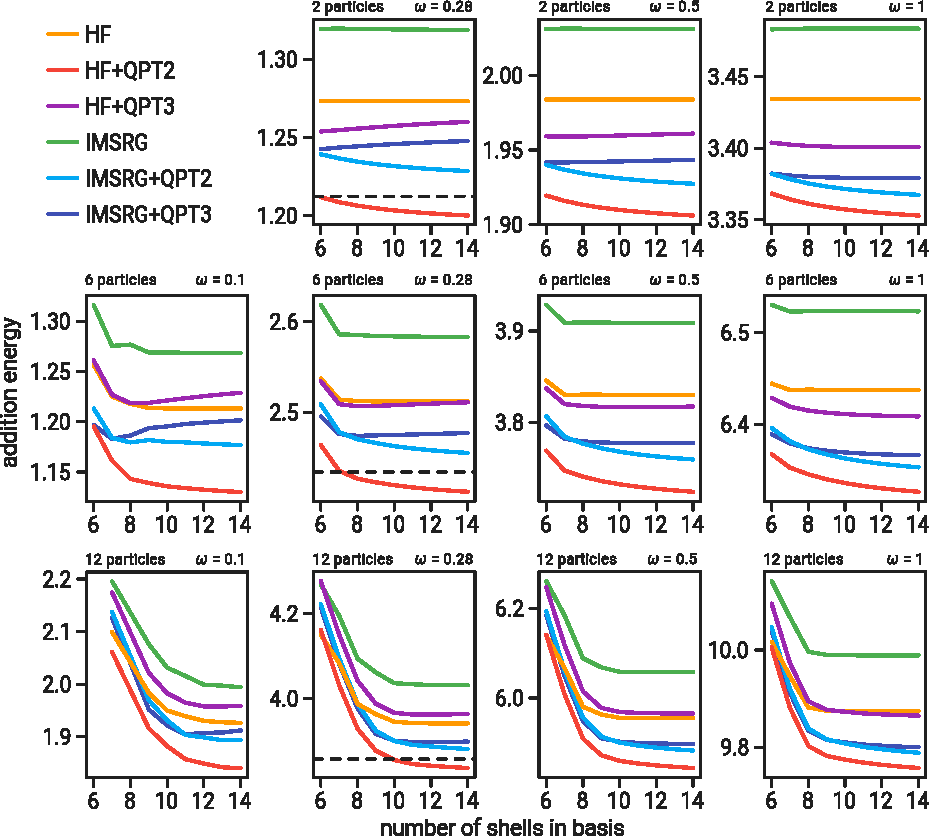
\includegraphics[width=0.8\textwidth]{fig-add}
  \caption{Addition energies.}
  \label{fig:add}
\end{figure}

\begin{figure}
  \centering
  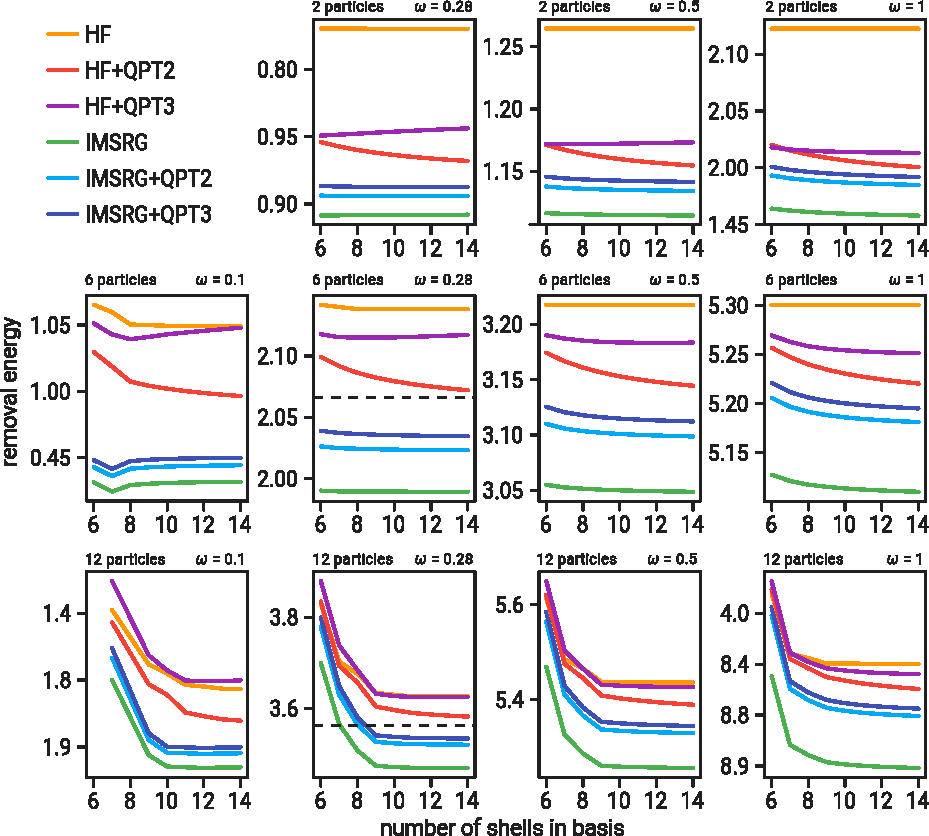
\includegraphics[width=0.8\textwidth]{fig-rm}
  \caption{Removal energies.}
  \label{fig:rm}
\end{figure}

\begin{figure}
  \centering
  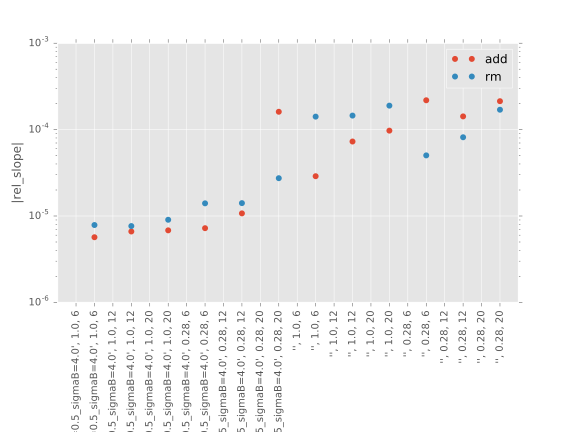
\includegraphics[width=0.8\textwidth]{fig-rel-slopes}
  \caption{Comparison of the rate of convergence for various modifications to the Coulomb interaction.  The key observation from this plot is that the short-range part of the interaction has a strong impact on the convergence, whereas the long-range tail has little effect.}
  \label{fig:rel-slopes}
\end{figure}

[[Sarah's discussions on ground state energy are absent :(]]
In this section, we discuss the IM-SRG results for the ground-state energies of closed-shell systems.  We start with the Wegner generator in subsection [[??]].  Numerical instabilities in the integration process, as well as a rather slow convergence as function of the number of oscillator shells, favors the use of a Hartree-Fock basis and the Coulomb interaction.  Since higher correlations still lead to stiff equation systems, we change in subsection [[??]] to the White generator. In particular, we give an overview of the IM-SRG(2) ground state energies for closed-shell systems up to $N=42$ particles and compare with other \textit{ab initio} many-body methods.

[[...]]


The discrepeancy between IM-SRG results and the exact result is due to a combination of two factors: inadequate basis set, and operator truncation.
The former can be reduced by increasing the number of shells, and can be further alleviated by extrapolation techniques.

Both IM-SRG and MP2 improve the accuracy the result dramatically over the more primitive HF.  (It may help to add plots *without* HF.)

[[TODO: add FCI, CCSD results to GS energy plots]]

\subsection{Comparison between methods}

\subsubsection{Ground state energy}

In Figure \ref{fig:gs} we display a selection of ground state energies calculated using the Hartree-Fock method, second-order (M\o ller-Plesset) perturbation theory (MPPT), and IM-SRG.  The exact result from diffusion Monte Carlo (DMC) is also shown as a dashed line \cite{PhysRevB.84.115302}.

Both perturbation theory and IM-SRG add corrections in addition to the Hartree-Fock results to recover the correlation energy and they do quite well in recovering the correlation energy in the system.  Compared with MPPT, IM-SRG generally converges faster, although does not always converge to the DMC result.  Generally speaking, IM-SRG is closer to the DMC result as the number of particles increases.

There are a few cases where the IM-SRG over-corrects the result, leading to a ground state energy that is lower than the exact result.  This is not unexpected given that, unlike Hartree-Fock, IM-SRG is non-variational in the presence of operator truncations, which cause small unitarity violations.  Overcorrection tends to occur when the number of particles is few, or the frequency is very low (high correlation).  However, MPPT does not do much better in the high frequency regimes as it often converges slower than IM-SRG.

The operator truncations in the evaluation of the commutator is one of the two sources of discrepancy between IM-SRG and exact results.  The other source is that of basis truncation, which limits the size of the Hilbert space that can be explored by the method.  Unlike operator truncation, which is difficult to overcome as it increases the computational cost exponentially, increasing the basis comes a cost of about $O(n^2 N^4)$ for IM-SRG(2) with the White generator,\footnote{This result holds for any generator whose two-body part contains only pphh- and hhpp-type matrix elements.} [[cite Heiko?]] where $N$ is the total number of states in the single-particle basis and $n$ is the number of particles.  In practice, the scaling cost is usually lower as the conserved symmetries allow the Hamiltonian to be partitioned into blocks.

\subsubsection{Addition and removal energies}

For our addition and removal energy calculations, the results are summarized in Figure \ref{fig:add} and Figure \ref{fig:rm} respectively.  The figures show the the addition/removal energies for Hartree-Fock, combined with IM-SRG and/or QDPT (Hartree-Fock is always included, as usual) [[better way to explain this? the figure labels are somewhat misleading too]].  The DMC results are also shown via dashed lines where they are known.

From these results, we see that the QDPT corrections add a substantial contribution to the results of both Hartree-Fock with and without IM-SRG.  [[quantify ``substantial'' numerically]]

Interestingly, the addition energy of Hartree-Fock with second-order QDPT appears to surpass the accuracy of that of IM-SRG with second-order QDPT.  This is likely coincidental, as the third-order QDPT dramatically worsens the result.

Both Hartree-Fock and IM-SRG results worsen as the frequency decreases, which is not unexpected since the correlations become much more dominant.  The Hartree-Fock appears to perform much worse, however, as the results converge much more slowly as the number of shells increases.

We also note that IM-SRG with 2 particles and a frequency 0.1 generally fail to give any result as the ODE solver eventually leads to divergence [[Why?]]  This seems to be a quirk isolated to this particular system and does not usually occur in other systems.

[[---]]

\subsection{Rate of convergence}

When the tail part of the convergence plots are magnified about a factor of ten or so [[double-check this number]], we noticed that the addition and removal energies are still drifting somewhat [[quantify how much]], hinting that the convergence rate is probably not exponential.

To investigate the rate of convergence, we tested our methods against a modified form of the Coulomb interaction, parametrized by two lengths $\sigma_{\mathrm{A}}$ and $\sigma_{\mathrm{B}}$ that characterize the range of the interaction:
\begin{align}
  V_{\sigma_{\mathrm{A}}, \sigma_{\mathrm{B}}}(r) \equiv \frac{(1 + c)^{1 - 1/c}}{c} \left(1 - \E^{-r^2 / (2 \sigma_{\mathrm{A}}^2)}\right) \E^{-r^2 / (2 \sigma_{\mathrm{B}}^2)} \frac{1}{r}
\end{align}
where $c \equiv \sqrt{\sigma_{\mathrm{B}} / \sigma_{\mathrm{A}}}$.  The coefficient is defined to ensure the peak of the envelope remains at unity.  By setting $\sigma_{\mathrm{A}} = 0$ and $\sigma_{\mathrm{B}} = \infty$ one recovers the original Coulomb interaction.  By increasing $\sigma_{\mathrm{A}}$ one can reduce the short-range part of the interaction, and analogously by increasing $\sigma_{\mathrm{B}}$ one can reduce the long-range part of the interaction.  For our numerical experiments we consider the following four combinations of $(\sigma_{\mathrm{A}}, \sigma_{\mathrm{B}})$: $(0, \infty)$, $(\frac{1}{2}, \infty)$, $(0, 4)$, $(\frac{1}{2}, 4)$.

To analyze the convergence as function of the number of shells $K$, we use a simple but approximate metric, the \textit{relative slope} at $K = 15$:
\begin{align*}
  \rho_{15}(\varepsilon) \equiv \frac{\varepsilon_{K = 15} - \varepsilon_{K = 14}}{\varepsilon_{K = 15}}
\end{align*}
For the systems we have selected, at $K = 15$ the addition and removal energies have essentially reached the asymptotic behavior (by visual inspection), thus $\rho_{15}$ gives a crude measure of the rate of convergence as a relative quantity independent of the energy unit, allowing it to be meaningfully compared between systems with different interactions and different particle numbers.  The results are plotted in Figure \ref{fig:rel-slopes}.

Analyzing the figure, we observe that the reducing short-range part of the interaction improves the rate of convergence greatly -- the relative slope has saturated and reached the precision of the ODE solver -- whereas eliminating the long-range part of the interaction had very little effect.  This demonstrates that the main cause of the slow convergence lies in the highly repulsive, short-ranged part of the interaction, which leads to the presence of nondifferentiable cusps (the so-called \textit{Coulomb cusps}) in the exact wave functions that are difficult to reproduce exactly using linear combinations of the smooth harmonic oscillator wave functions.

The figure also tells us that the convergence is negatively impacted at lower frequencies and, to a lesser extent, by the number of particles.  Both are expected: lower frequencies increase the correlation in the system, while higher number of particles naturally require more shells to converge.

We also note that the behavior of addition energies versus removal energies tend to be similar, and which one converges faster fluctuates from system to system.

\subsection{Extrapolation}

As suggested by Kvaal in \cite{PhysRevB.80.045321}, the asymptotic convergence of the wave function can be approximately described by a power law model: [[assuming I understood his paper correctly]]
\begin{align*}
  \Delta E \propto K^{-\beta}
\end{align*}
where $\Delta E$ is the error in the energy, $K$ is the number of shells in the single-particle basis, and $\beta$ is some positive real exponent.  Essentially, the \textit{smoothness} of the exact wave function determines the rate of the convergence: the more times the exact wave function can be differentiated, the higher the exponent $\beta$.

It is difficult to ascertain what $\beta$ is \textit{a priori}, but based on Kvaal's results $\beta$ is expected to be below $5$ for quantum dot systems.  To determine this from our numerical calculations, we perform a curve using the following power-law model:
\begin{align} \label{eq:power_law_model}
  E = \alpha K^{-\beta} + \gamma
\end{align}
As with most nonlinear curve fits, it is often fairly sensitive to the initial parameters.  To extract the initial parameters, we first do a linear fit on $\ln (\partial E / \partial K)$ against $\ln (K)$:
\begin{align*}
  \ln \left(\frac{\partial E}{\partial K}\right) = \ln(\alpha) - \beta \ln(K)
\end{align*}
The derivative is approximated using finite differences of adjacent data points:
\begin{align*}
  \frac{\partial E}{\partial K} \approx E\left(K + \frac{1}{2}\right) - E\left(K - \frac{1}{2}\right)
\end{align*}
The process of calculating a derivative amplifies the noise, but linear fits do have the strong advantage of being very reliable to fit -- there is little concern about being stuck in a local minimum -- as well as making the results easy to judge by visually.  Of course, linear fits do not weigh the individual contributions equally, thus a more accurate nonlinear curve fit is required afterward.

We use the results as inputs for a power-law fit of $E$ against $K$, which is not as sensitive to noise.  We do require a guess for the infinite-basis energy $\gamma$, which we estimate by fitting \eqref{eq:power_law_model} while the parameters $\alpha$ and $\beta$ are fixed to the initial guesses.  Finally, we do a fit with all three parameters free to vary.

There is still one additional tuning knob for this model that is not explicitly shown in \eqref{eq:power_law_model}: the range of data points taken into consideration.  Since the model describes the \emph{asymptotic} behavior, we do not expect the fit to produce good results when the energy is still far from convergence.  To remedy this, we restrict ourselves to fitting only the last few data points within some chosen range.  If range is too large, then the non-asymptotic behavior would perturb the result too much, whereas if the range is too small, the noise will obscure the result.  This part is tuned by hand based on observations of the log-log plot: we expect the asymptotic region to lie more or less on a straight line.

[[Idea for further exploration: see how much the extrapolation improves the result, and see what happens as we increase the number of shells included in the fit on the right/upper bound.]]

[[Hypothesis for the poor HF fits: either it's decaying so fast that it quickly becomes dominated by the precision of the calculation, or it's exponential.]]

\section{Conclusions}
\label{sec:conclusions}

We have demonstrated the use of various many-body theories -- Hartree-Fock method, M\o eller-Plesset perturbation theory, in-medium similarity renormalization group, and quasidegenerate perturbation theory -- to calculate ground state as well as addition and removal energies of two-dimensional circular quantum dots up to 56 [[make sure the figure/data for 56 particles stays]] particles.  We showed that these methods, when combined, can provide a good, approximate description of the systems at moderate cost compared to near-exact but much more expensive methods such as FCI and DMC.

Two different generators, Wegner and White generators, were used [[T/F?]] to perform the calculations.  It was observed that the Wegner generator results in stiff equation systems, whereas the White generator has much better numerics and is computationally more efficient.[[make sure this is this elaborated in the Results section]] Moreover, we found out that the use of an Hartree-Fock basis improves numerical stability enormously.

For ground state energy, we showed that the convergence of IM-SRG is generally faster than that of MPPT, and the results are typically closer to the the near-exact results.  Similar to previous FCI \cite{2008arXiv0810.2644K} and CCSD \cite{PhysRevB.84.115302} calculations, the use of an effective interaction improves convergence of the ground state energy as function of the number of oscillator shells.  [[delete or keep: For more than six particles, we lie in all cases closer to the DMC result than corresponding CCSD calculations do.]]

For addition and removal energies, we found that IM-SRG improves their rate of convergence both as the order of perturbation theory increases and as the number of shells increases.

There are several directions in which the calculations may be improved.  One can attempt to improve the IM-SRG approximation by incorporating some of the missing higher-body terms in the commutator.  This would also provide some insight into the rate of convergence with respect to the operator truncation, providing a sense of how large the truncation error is.  While a full 3-body treatment of IM-SRG would be extremely costly, it is possible implicitly track for a portion of the induced 3-body forces by computing certain diagrams that are either lower cost or could be approximated at lower cost [[Ref?]].

As noted earlier [[not yet written]], the application of IM-SRG eliminates a large portion of the QDPT diagrams, which is beneficial as it increases the efficiency of the QDPT calculations.  However, many of these diagrams can also be eliminated further through an infinite resummation scheme [[Good refs for this?]], which would further reduce the number of diagrams in QDPT, especially those of lower order, whic would likely increase the accuracy of the result.

It would also be useful to investigate how the results obtained with finite
number of shells in the basis are related to those obtained with an infinite
number of shells in the basis.  [[Ref: IR/UV extrapolation]] With a
good theoretical foundation, a model of how the observables converge with
respect to the size of the basis may be used to extrapolate the results to
infinite-basis limit.  This would also enable us to perform cheaper
calculations with fewer shells and optimistically extrapolate results for
large systems that would be otherwise infeasible to compute.

We note that this calculation was done entirely using the traditional approach of using a high-order ODE solver to solve the flow equation.  A new technique developed by T. D. Morris \cite{PhysRevC.92.034331} uses an alternative approach that obviates the need for a high-order ODE solver, leading to much more efficient computations and also allowing operators of other observables to be evolved with greater ease.  Implementing this approach would be beneficial as it would allows us to study the accuracy and convergence of other observables beyond energy and energy differences.

Implementation-wise, our current code constructs the two-particle states as simple Slater determinants of their one-particle states.  This approach is often referred to as \textit{m-scheme} in nuclear physics.  It is a simple approach and works well for general systems, but it does not fully exploit the symmetries in the quantum dot system, since not only is spin projection $\hat S_z$ conserved, but squared spin $\hat S^2$ too.  A more efficient approach is to couple the spins of the single-particle states to form two-particle states with good $\hat S^2$, an approach analogous to \textit{j-scheme} in nuclear physics.  Combining this with the spherical tensor symmetries of the Hamiltonian, this can reduce the amount of computation required in this system via the Eckart-Wigner theoerem, albeit at the cost of increasing the implementation complexity.

A more technical issue is its lack of parallelization: currently, the code makes very little use of parallelism and therefore does not scale well on modern clusters.  Parallelism would allow the workload and memory resources to be divided over multiple computing nodes, allowing larger systems to be explored, but this must be weighed carefully against the costs of communication, which can be severe if the algorithm is chosen poorly.

Eventually, we plan to apply these theoretical and technical enhancements not only to the study of quantum dots, but to the studies of nuclear and atomic systems, opening up an even larger range of applications.

\begin{acknowledgments}
  This work was supported by the National Science Foundation Grant No.~PHY-1404159 (Michigan State University) and by the Research Council of Norway under contract ISP-Fysikk/216699.  This research used computational resources of the Notur project in Norway.  We thank Christoffer Hirth, Simen Kvaal and Veronica Olsen for several discussions.
\end{acknowledgments}

\bibliographystyle{\mybibstyle}
\bibliography{paper}
\end{document}
